\documentclass{article}

\usepackage[T1]{fontenc}    %Schriftart des Dokumentes
\usepackage[ngerman]{babel} %Dokumentensprache, hier Deutsch
\usepackage{amsmath, amssymb, stmaryrd} %mathematische Schriftzeichen
\usepackage{mathtools}
\usepackage{graphicx} %Einfügen von Grafiken
\usepackage{wrapfig}
\usepackage{bm}
\usepackage{subfig}
\usepackage{newclude}
\usepackage{pdfpages}

\setlength{\parindent}{0pt} %Einrückung von Absätzen auf null gesetzt
\setlength{\parskip}{10pt} %Abstand zischen Absätzen auf 10pt gesetzt

\title{Versuch 213: Kreisel}
\author{Matthias Kuntz}
\date{27.02.2024}

\renewcommand*\contentsname{Zusammenfassung}

\begin{document}

\maketitle

\tableofcontents

\newpage

%-------------------------EINLEITUNG-------------------------
\section{Einleitung}

Eine Frage, die sich wohl viele Menschen von klein auf stellen werden, ist, warum ein rotierender Kreisel, selbst wenn man diesen etwas anstößt, nicht umfällt. Was genau unterscheidet ein rotierendes Objekt von einem nicht rotierenden und wie sorgt die Rotation für eine scheinbar wie von Geisterhand kommende aufrechterhaltende Kraft? Um all diese Fragen soll es in diesem Versuch gehen, indem wir verschiedene Bewegungen einer als Kreisel fungierenden Kugel in einem Luftkissenbecken untersuchen. Denn die Kreisel sind nicht nur relevant für unser aller liebstes Kinderspielzeug, sondern haben weit größere Bedeutung in der realen Welt. Allein der Fakt, dass unsere Erde selbst ein riesiger Kreisel ist, der um seine Achse rotiert und präzediert, später mehr zur allgemeinen Terminologie, ist ein Zeichen für die grundlegende Relevanz von Kreiselphänomenen der Physik in praktisch allen Teilgebieten.

\subsection{Physikalische Grundlagen}

\subsubsection{Der kräftefreie, symmetrische Kreisel}

Als Kreisel bezeichnet man jeden starren Körper, der sich um einen festen Punkt dreht. Ist dieser dabei in seinem Schwerpunkt gelagert heißt er kräftefrei und wenn zwei Hauptträgheitsmomente gleich sind ist er symmetrisch. Bei Kreiseln gibt es drei charakteristische Achsen: Die Symmetrieachse des Kreisels, genannt Figurenachse $\Vec{F}$, die raumfeste Drehimpulsachse $\Vec{L}$ sowie die Drehachse $\Vec{\omega}$. Der einfachste Fall ist, wenn alle drei bei einer Rotation zusammenfallen, zu sehen in Abbildung \ref{fig:kräftefrei_symm_bew} links. Allgemein ist die Bewegung aber etwas komplizierter. Verpasst man dem aufrecht rotierenden Kreisel beispielsweise einen leichten Schlag, so kann man die drei Achsen trennen und der Kreisel beginnt eine komplexe Taumelbewegung, genannt Nutation, zu sehen in Abbildung \ref{fig:kräftefrei_symm_bew} mittig. Hierbei bleibt $\Vec{L}$ zeitlich und räumlich konstant. Die Figurenachse $\Vec{F}$ beginnt jedoch auf einem Kegelmantel, dem Nutationskegel, mit der Nutationsfrequenz $\Vec{\omega}_N$ um die raumfeste Drehimpulsachse $\Vec{L}$ zu rotieren und sich mit der Eigenrotation $\Vec{\omega}_F$ um sich selbst zu drehen. Somit ist auch die resultierende Drehachse nicht konstant und man spricht nur noch von der momentanen Drehrichtung $\Vec{\omega}$ des Kreisels zu einem bestimmten Zeitpunkt.

Eine gute Visualisierung bietet Abbildung \ref{fig:kräftefrei_symm_bew} rechts. Stellt man sich $\Vec{F}$ als Symmetrieachse eines Körperkegels und $\Vec{L}$ als die eines raumfesten Raumkegels vor, so lässt sich die Bewegung beschreiben indem man sich vorstellt, dass sich der Körperkegel um den Raumkegel herumrollt. Die Drehrichtung $\Vec{\omega}$ ergibt sich dann immer aus der Berührungslinie der beiden Kegel. 

\begin{figure}[!h]
    \centering
    \includegraphics[width=0.9\textwidth]{graphics/kräftefrei_symm.png}
    \caption{Verschiedene Bewegungen des kräftefreien, symmetrischen Kreisels [Quelle: PAP2.1 Skript, S.20, 05.03.2024]}
    \label{fig:kräftefrei_symm_bew}
\end{figure}

\newpage

Gut zu erkennen ist hierbei, dass die drei Achsen getrennt sind, aber immer noch zu jedem Zeitpunkt in einer Ebene liegen. Somit können wir mithilfe von Abbildung \ref{fig:krf_symm_geom} links die momentane Winkelgeschwindigkeit $\Vec{\omega}$ immer in einen Nutationsanteil $\Vec{\omega}_N$ und einen Anteil der Eigenrotation der Figurenachse $\Vec{\omega}_F$ unterteilen: 

\begin{equation}
    \Vec{\omega} = \Vec{\omega}_N + \Vec{\omega}_F
\end{equation}

Analog können wir, siehe Abbildung \ref{fig:krf_symm_geom} rechts, Drehimpuls und momentane Winkelgeschwindigkeit in die Komponenten der x- und z-Richtung unterteilen, um den Betrag der Nutationsfrequenz $\omega_N$ zu bestimmen:

\begin{equation}
    \begin{split}
        \omega_x &= \omega_N \sin{\theta} \\
        L_x &= L \sin{\theta} = I_x \omega_x \\
        &\Rightarrow \omega_N = \frac{L}{I_x}
    \end{split}
\end{equation}

Für kleine Nutationsbewegungen, ergo für $\theta \ll 1$, können wir folgende Näherung machen:

\begin{equation}
    \begin{split}
        L &\approx I_z \omega \approx I_z \omega_F \\
        &\Rightarrow \omega_N \approx \frac{I_z}{I_x} \omega_F.
    \end{split}
    \label{eq:w_n-w_f}
\end{equation}

\begin{figure}[!h]
    \centering
    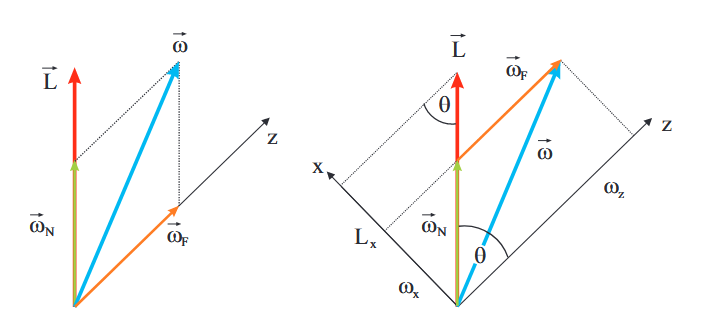
\includegraphics[width=0.9\textwidth]{graphics/krf_symm_zerleg.png}
    \caption{Geometrie der Nutationsbewegung [Quelle: PAP2.1 Skript, S.20, 05.03.2024]}
    \label{fig:krf_symm_geom}
\end{figure}

\phantom{.}

Bei diesem Versuch verwenden wir eine Stahlkugel, an der ein langer Stab angebracht ist, welcher die Nutationsbewegung sichtbar macht, siehe Abbildung \ref{fig:nutationskegel}. Zur Beobachtung der momentanen Drehachse verwenden wir eine auf die Figurenachse gesteckte Scheibe mit verschiedenen Farbsegmenten. Dadurch kann man beobachten, wie am Ort der momentanen Drehachse die einzelnen Farben der Sektorscheibe mit der Winkelgeschwindigkeit $\Omega$ (siehe Abbildung \ref{fig:kräftefrei_symm_bew}) durchlaufen werden. Man kann den Betrag von $\Omega$ mithilfe der Radien vom Körperkegel $r_{KK}$ und Raumkegel $r_{RK}$ sowie der Nutationsfrequenz $\omega_N$ bestimmen:

\begin{equation}
    \frac{\Omega}{\omega_N} = \frac{r_{RK}}{r_{KK}}.
\end{equation}

Das Ergebnis dieser Rechnung lautet:

\begin{equation}
    \begin{split}
        \Omega &= \frac{I_x - I_z}{I_x} \omega_F \\
        \iff I_x - I_z &= \frac{I_z}{\frac{\omega_F}{\Omega}-1}
        \label{eq:WinkegeschwOmega}
    \end{split}
\end{equation}

\begin{figure}[!h]
    \centering
    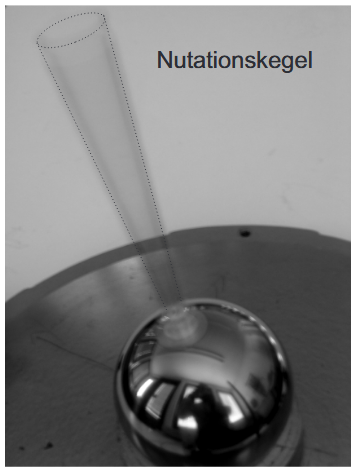
\includegraphics[width=0.4\textwidth]{graphics/nutationskegel.png}
    \caption{Nutationsbewegung der Figurenachse [Quelle: PAP2.1 Skript, S.21, 05.03.2024]}
    \label{fig:nutationskegel}
\end{figure}

\newpage

\subsubsection{Der schwere, symmetrische Kreisel} \label{Schw_Symm_Kreisel}

Verschiebt sich der Schwerpunkt des Kreisels, beispielsweise wie hier durch extra angebrachte Gewichte auf der Figurenachse, sodass dieser nicht mehr mit dem Unterstützungspunkt zusammenliegt, so ist es nun ein schwerer Kreisel. Wir wollen in diesem Versuch beim schweren Kreisel nur Bewegungen ohne Nutation beobachten. Die extra Gewichte $m$ üben aufgrund der Gewichtskraft ein Drehmoment auf den Kreisel aus:

\begin{equation}
    \Vec{M} = \Vec{l} \times m \Vec{g}.
\end{equation}

Hierbei ist $\Vec{l}$ der Vektor vom Unterstützungspunkt zu den Zusatzmassen auf der Figurenachse, siehe Abbildung \ref{fig:präzession} links. Dieses äußere Drehmoment sorgt nun für eine Änderung der Drehimpulsrichtung, nicht aber für einen Änderung von dessen Betrag. Dabei läuft der Drehimpulsvektor praktisch auf einem Kegelmantel um die z-Richtung, wobei er versucht der Gewichtskraft sozusagen seitlich auszuweichen. Das Resultat ist eine Kreiselbewegung genannt Präzession. Die Frequenz dieser Rotationsbewegung $\Vec{\omega}_P$ lässt sich nach Abbildung \ref{fig:präzession} rechts aus der zeitlichen Änderung des Präzessionswinkels $\phi$ folgendermaßen bestimmen:

\begin{equation}
        \omega_P = \frac{d \phi}{dt} = \frac{dL}{L \sin{\alpha} \ dt}.
\end{equation}

Verwenden wir wieder $L = I_z \omega_F$, so erhält man

\begin{equation}
        \omega_P = \frac{mgl}{I_z \omega_F}
        \label{eq:omegaP_omegaF}
\end{equation}

beziehungsweise allgemein:

\begin{equation}
     \Vec{M} = \Vec{\omega}_P \times \Vec{L}.
\end{equation}

Somit kann man sehen, dass die Präzessionsfrequenz unabhängig von der räumlichen Orientierung des Kreisels ist.

\phantom{.}

\begin{figure}[!h]
    \centering
    \includegraphics[width=0.9\textwidth]{graphics/präzession.png}
    \caption{Präzession eines Kreisels [Quelle: PAP2.1 Skript, S.22, 05.03.2024]}
    \label{fig:präzession}
\end{figure}

\phantom{.}

Wie bereits erwähnt gilt dies nur für präzidierende Kreisel ohne Nutation. Kommt eine Nutationsbewegung zur Präzessionsbewegung hinzu, so beginnt die Figurenachse eine deutlich kompliziertere "girlandeförmige" Bewegung. Da dies aber für diesen Versuch nicht von quantitativer Bedeutung ist, werden wir hier nicht weiter darauf eingehen.

\newpage
\subsection{Versuchsaufbau}

Das Hauptstück des Versuchsaufbaus ist der Luftkissenkreisel, genauer zu sehen in Abbildung \ref{fig:luftkissenkreisel}. Eine luftkissengelagerte Stahlkugel mit einem Aluminiumstab dient hierbei als Kreisel, wobei der Stab die Figurenachse sowie die $I_z$-Achse festlegt. Am Stabende ist ein Kugellager angebracht, an dem man die Orientierung des Stabs ohne größeren Einfluss auf die Frequenzen verändern kann. Die Kugel ist hierbei trotz des Stabs auf der Stabseite leichter, wodurch Extragewichte auf dem Stab angebracht werden müssen, damit dieser kräftefrei wird. Hierzu dient primär bei uns die eine Scheibe mit Reflektorstreifen.

Zusätzlich dienen ein Motor zur Antreibung des Kreisels und ein Stroboskob mit verschiedenen Scheiben, die auf den Stab gesteckt werden können, zur Bestimmung der Frequenzen. Der auf einer Scheibe angebrachte Reflektorstreifen kann dabei verwendet werden, um die Frequenz des Strobokobs der des Kreisels anzupassen und so dessen Drehfrequenz zu ermitteln. Zusätzlich werden noch Stoppuhren zur Messung der Umlaufzeiten verwendet.  

\phantom{.}

\begin{figure}[!h]
  \centering
  \subfloat[Übersicht der Materialien]{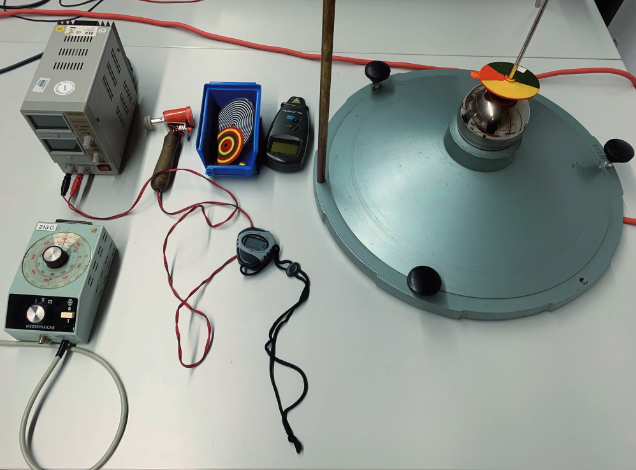
\includegraphics[width=0.48\textwidth]{graphics/aufbau.png}\label{fig:Aufbau_allg}}
  \hfill
  \subfloat[Aufbau des Luftkissenkreisels]{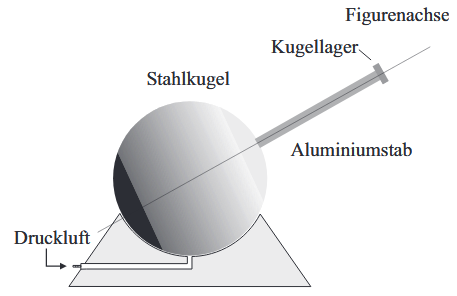
\includegraphics[width=0.48\textwidth]{graphics/luftkissenkreisel.png}\label{fig:luftkissenkreisel}}
  \hfill
  \caption{Versuchsaufbau [Quelle: PAP2.1 Skript, S.17 (a) \& 23 (b), 05.03.2024]}
  \label{fig:aufbau}
\end{figure}

%---------------VERSUCHSPROTOKOLL MIT MESSDATEN---------------
\newpage

\section{Versuchsprotokoll mit Messdaten}

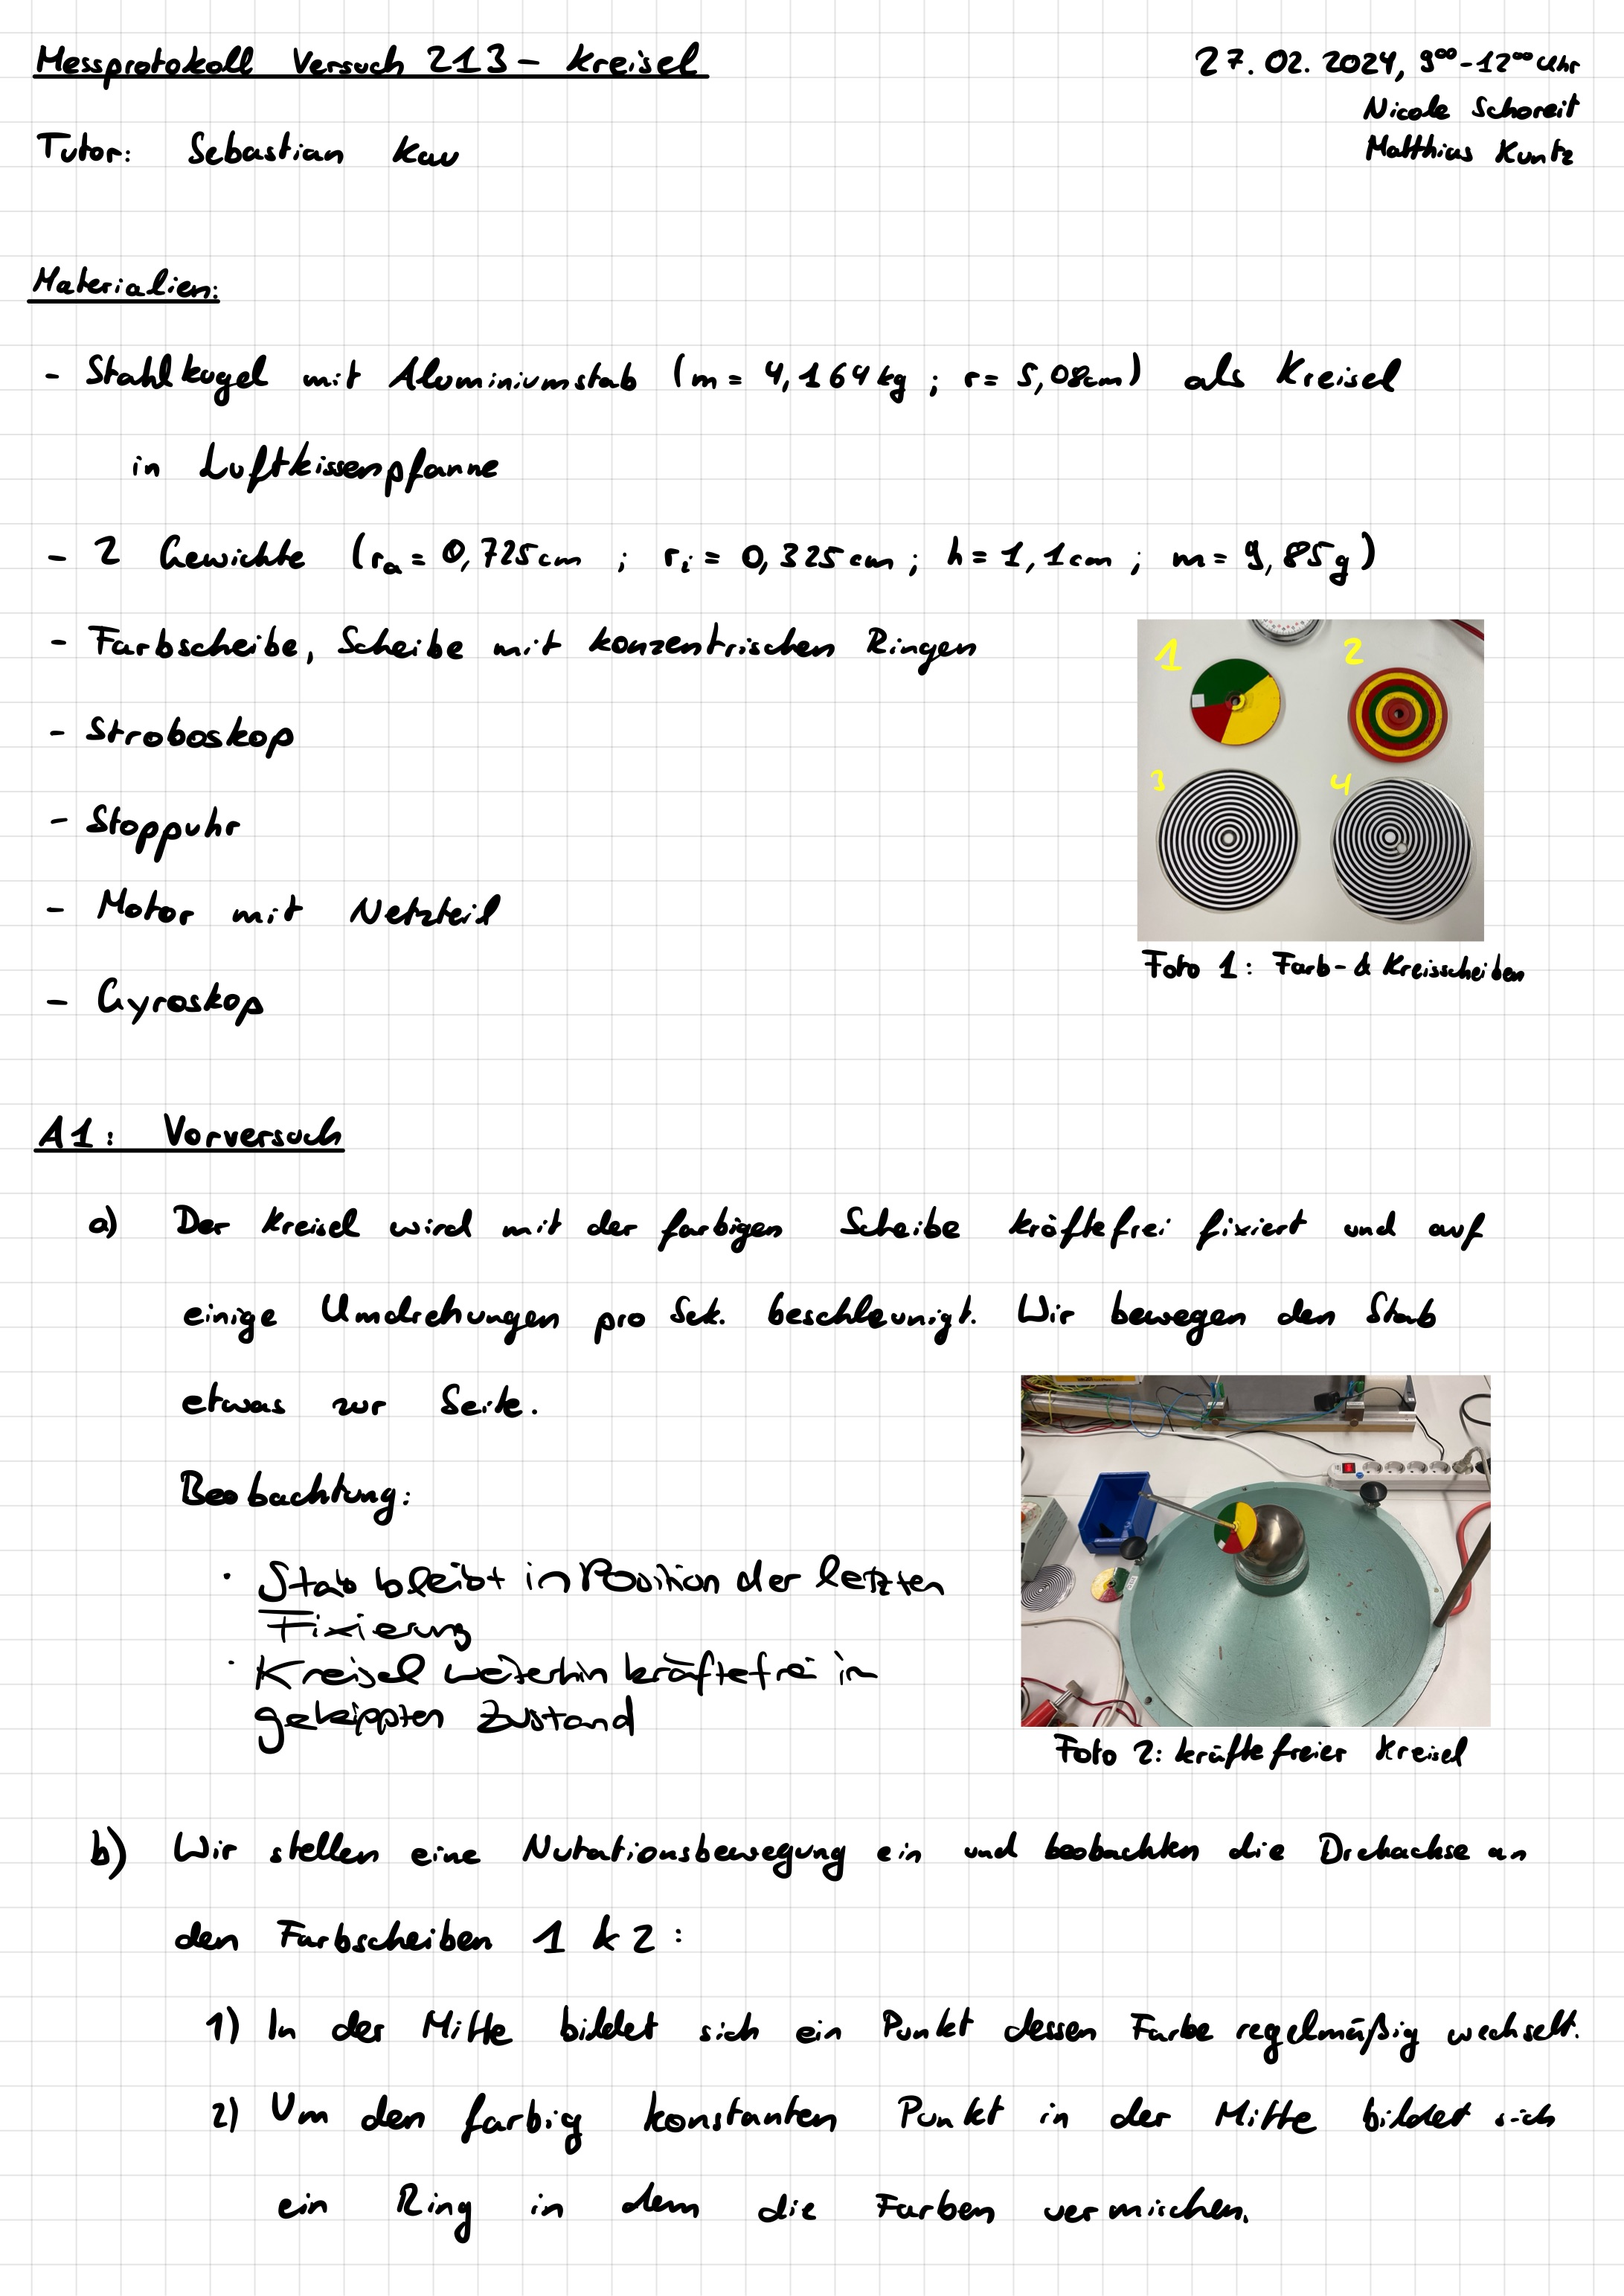
\includegraphics[width=\textwidth]{graphics/mess1.jpg}
\newpage
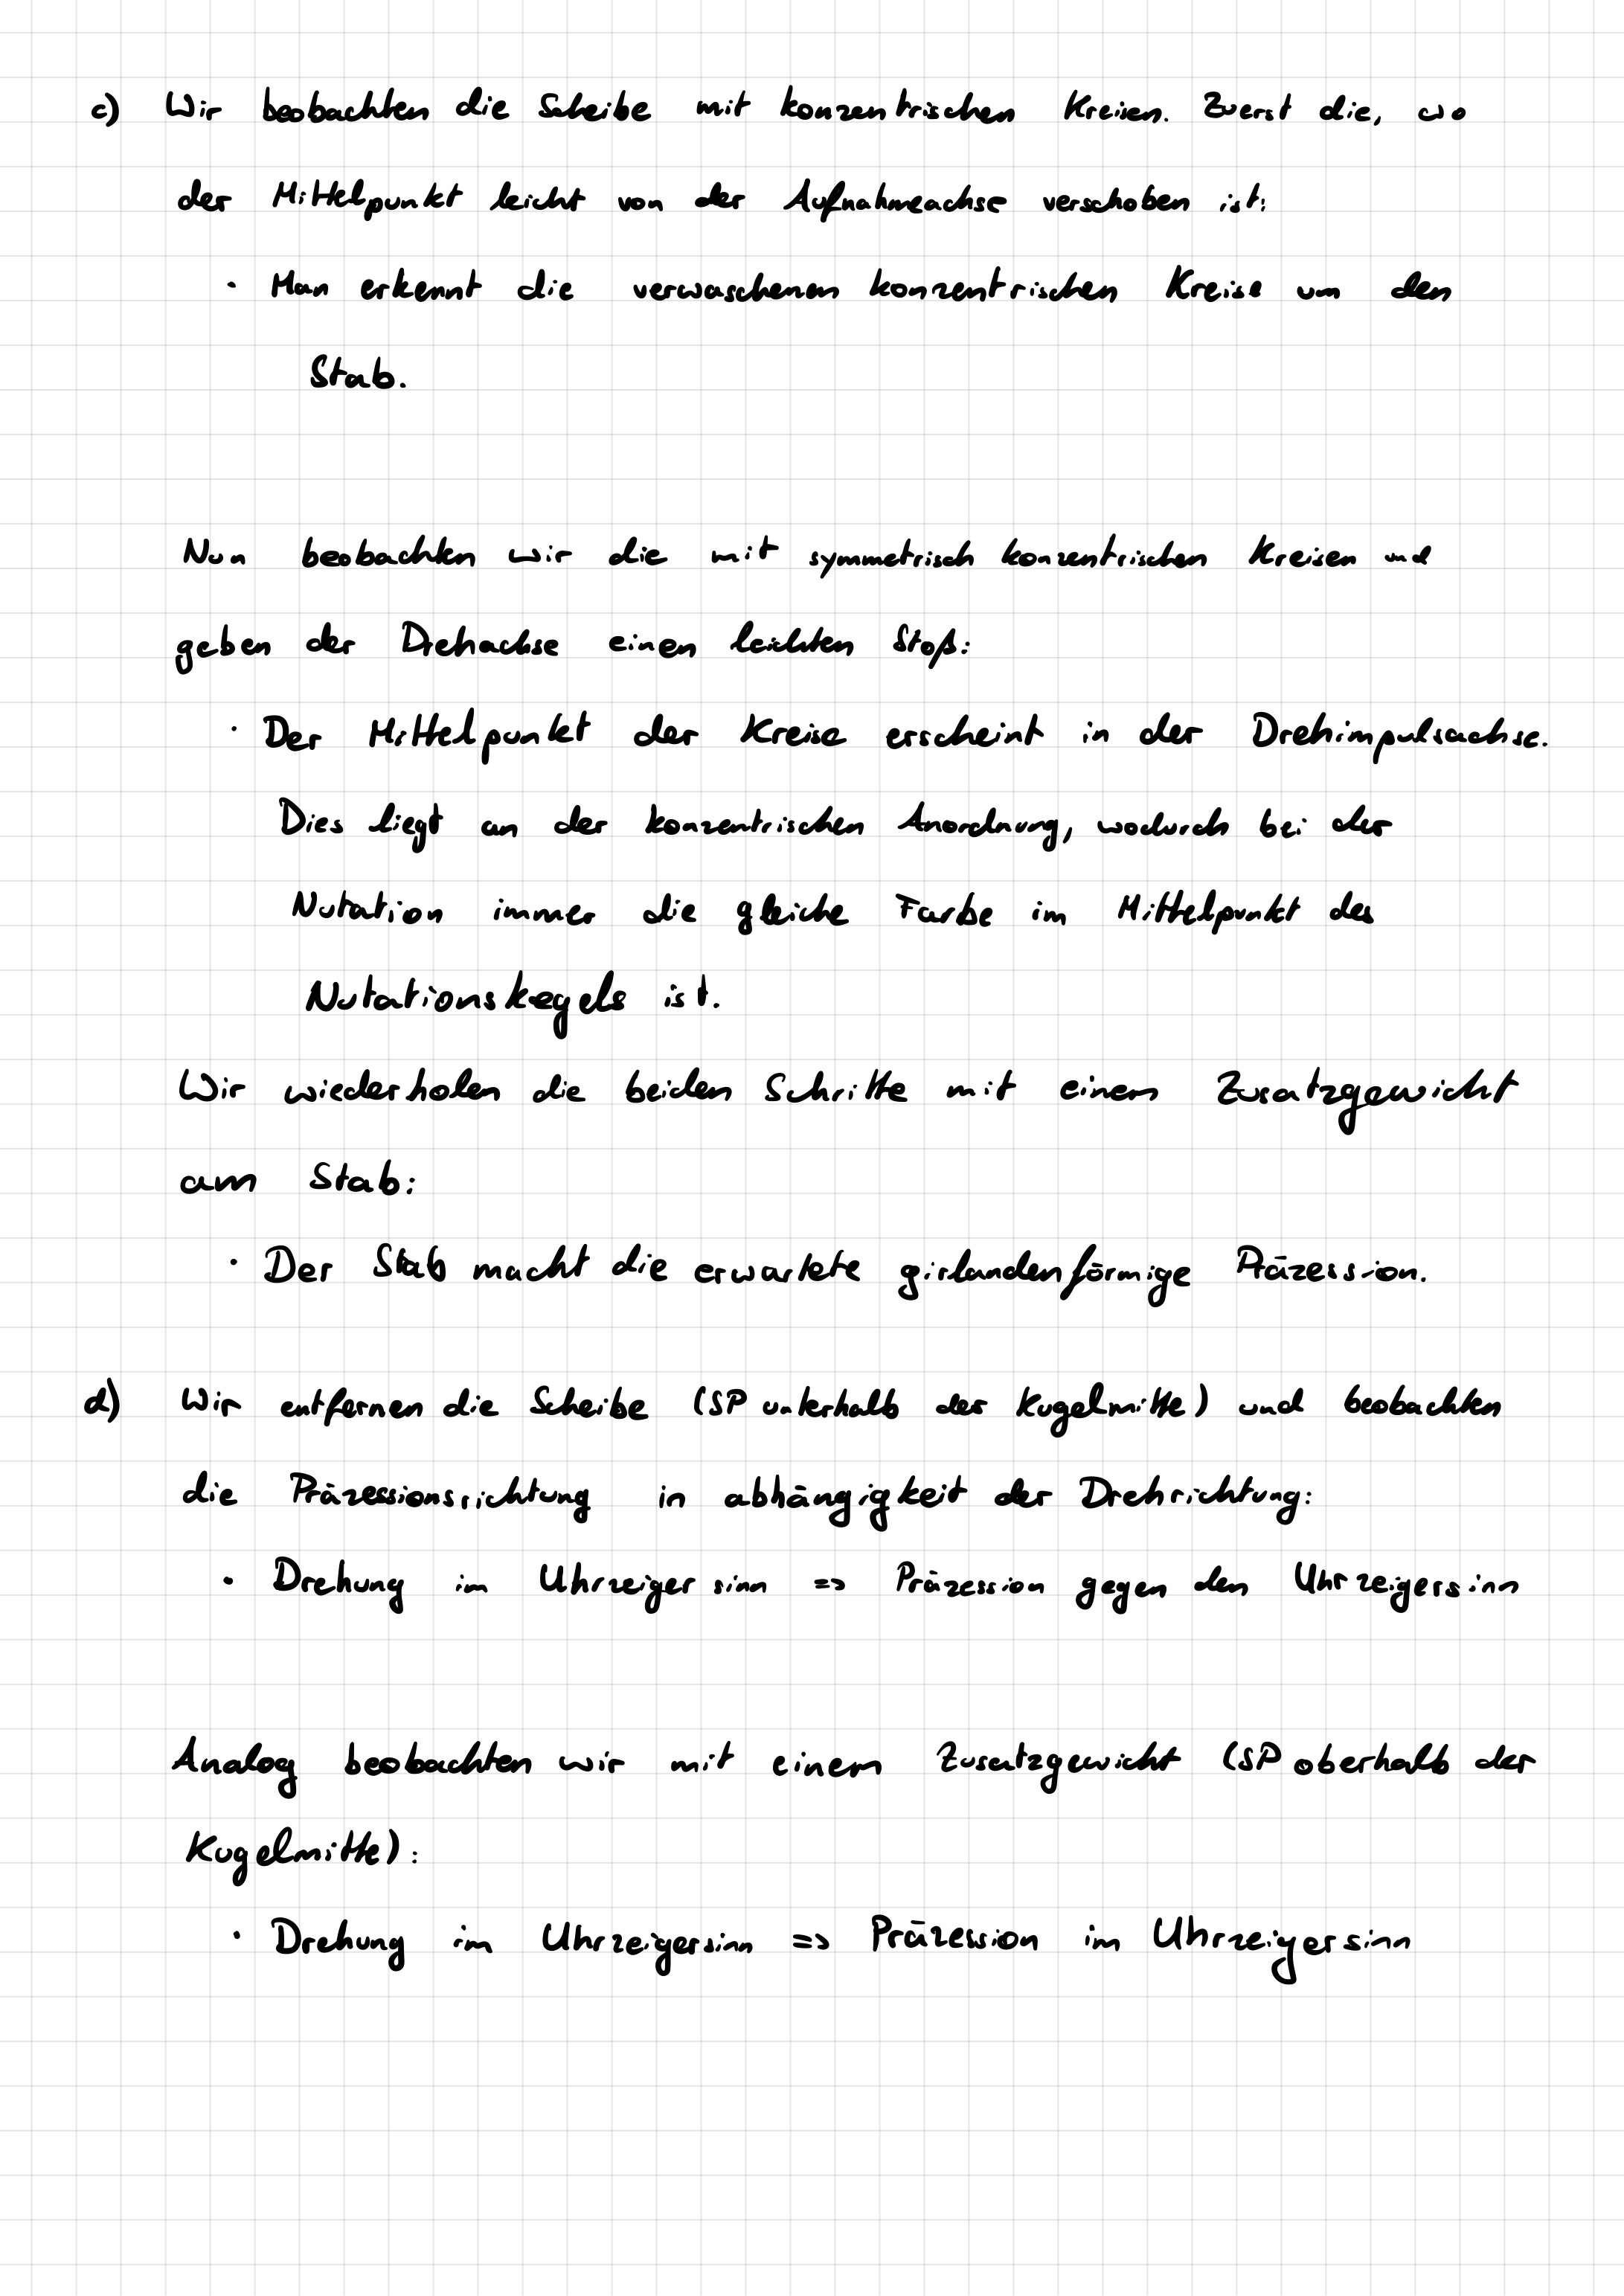
\includegraphics[width=\textwidth]{graphics/mess2.jpg}
\newpage
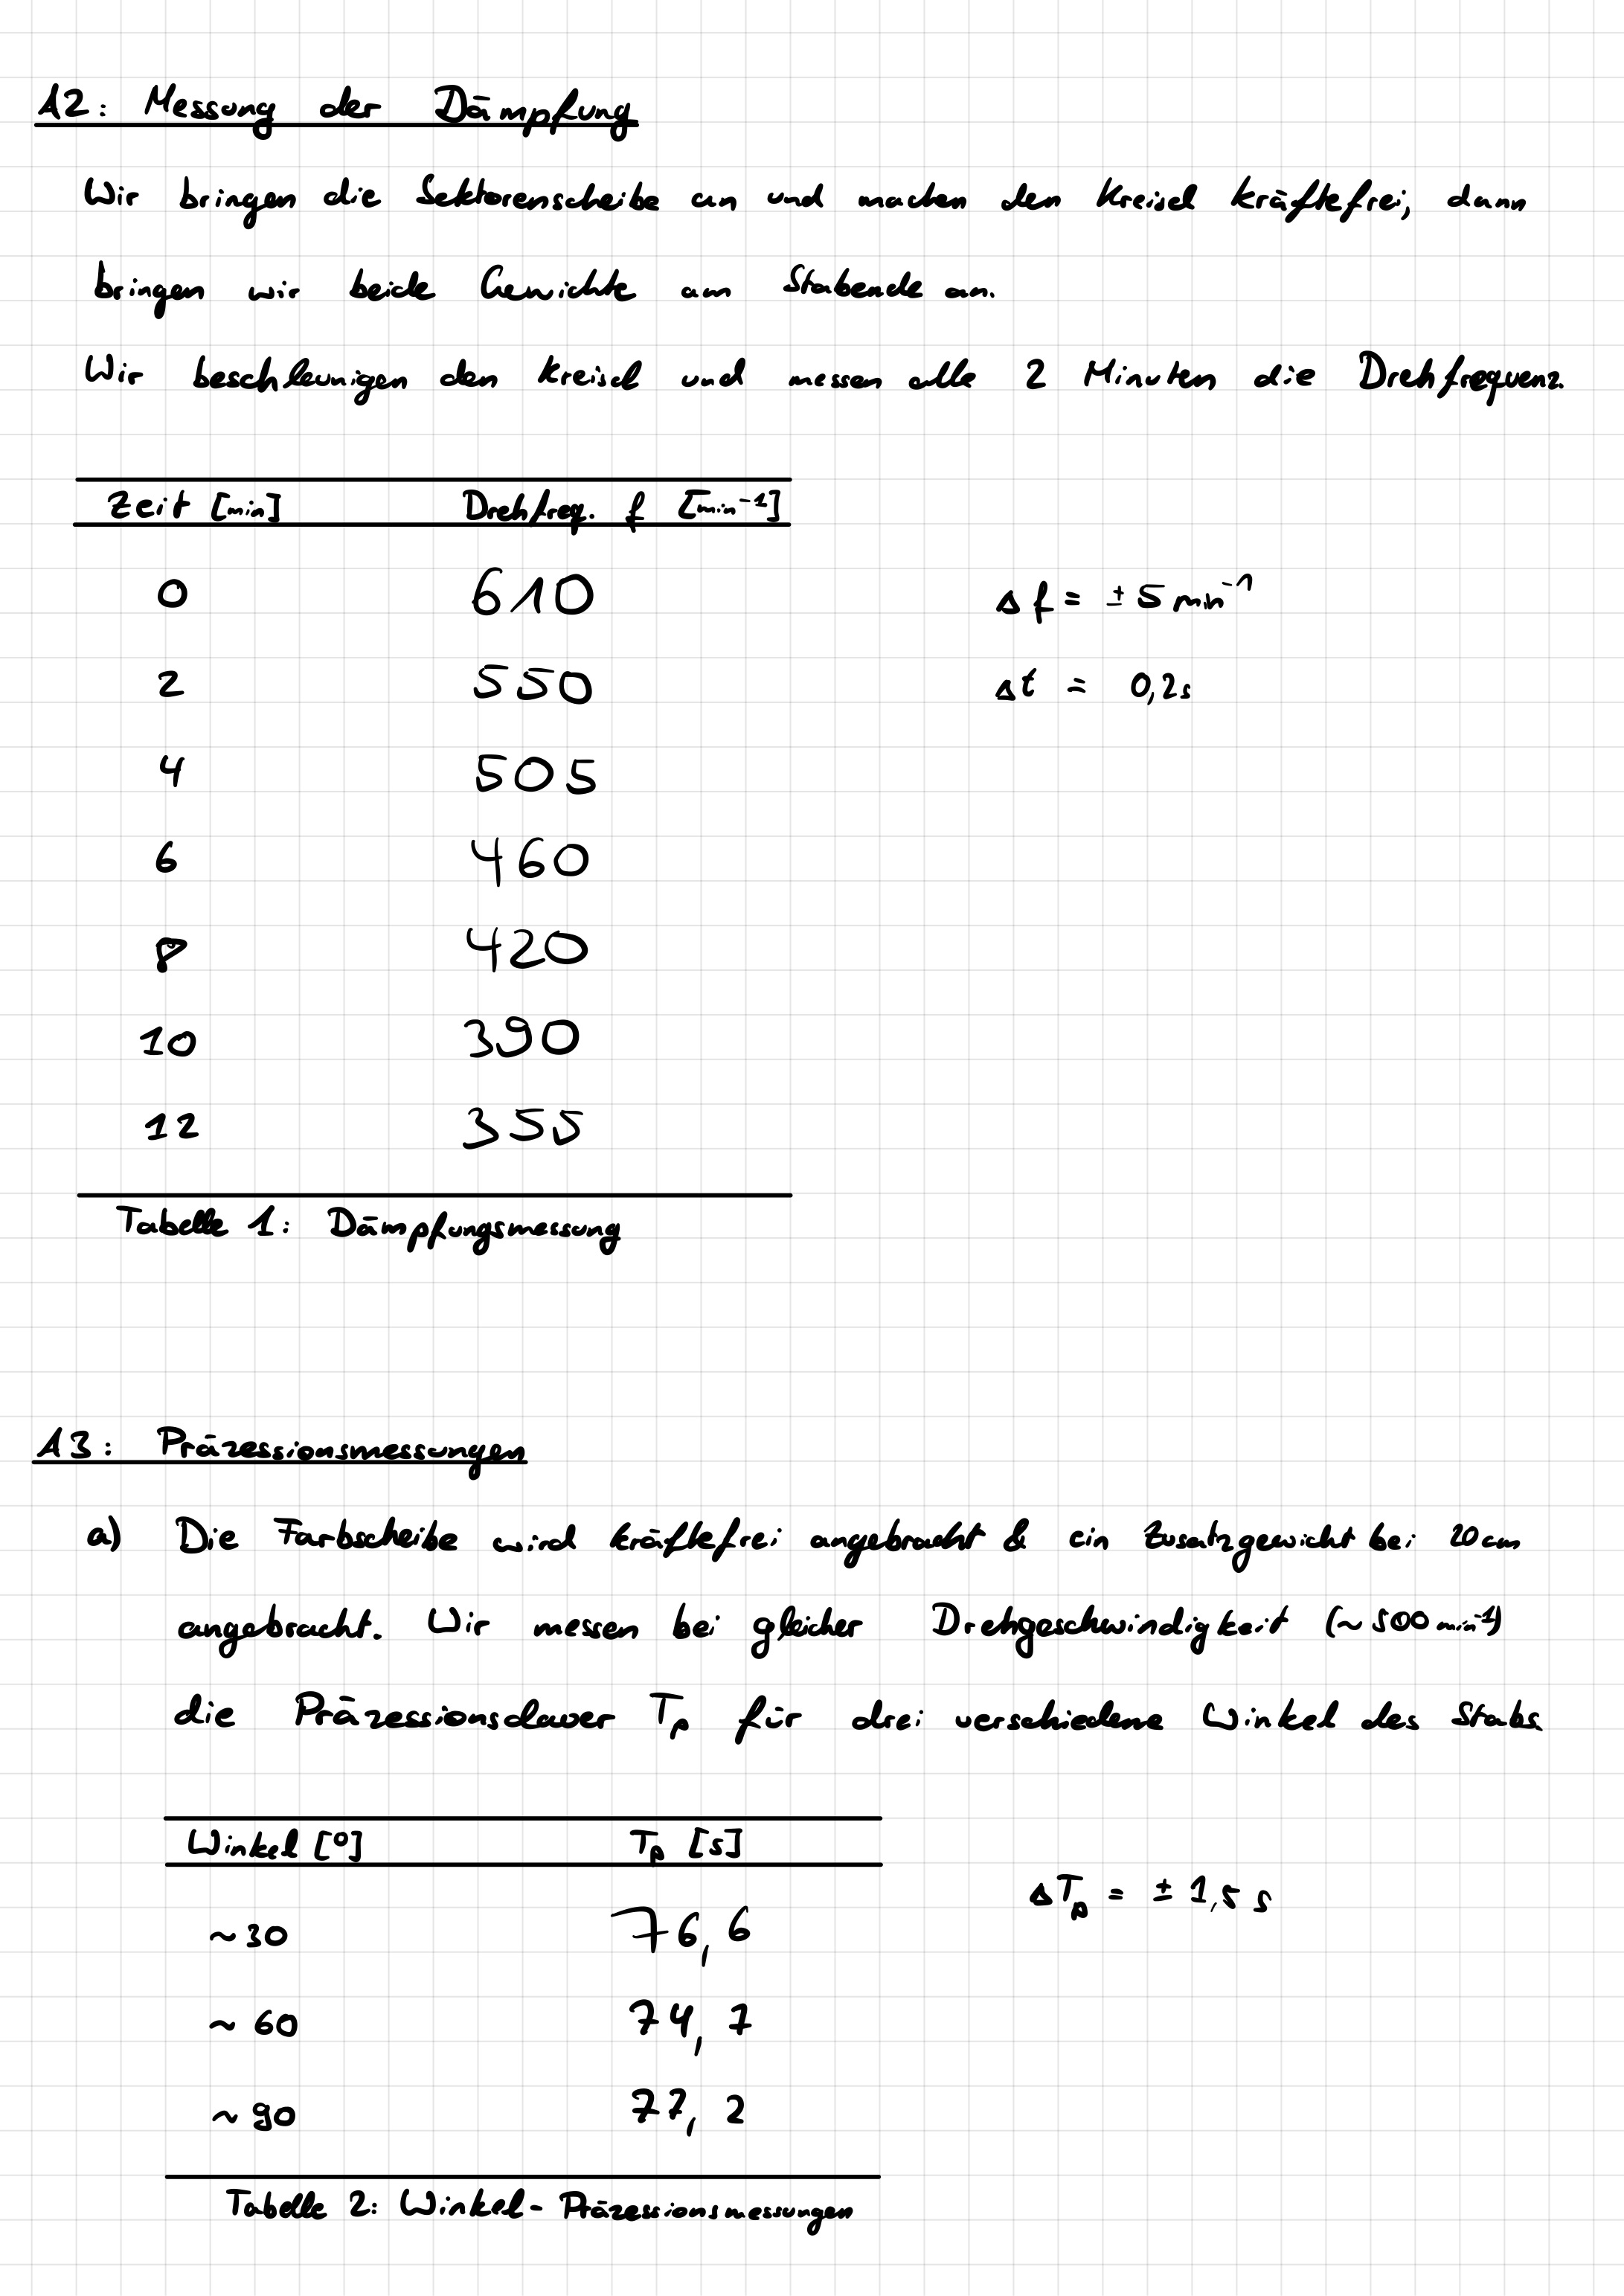
\includegraphics[width=\textwidth]{graphics/mess3.jpg}
\newpage
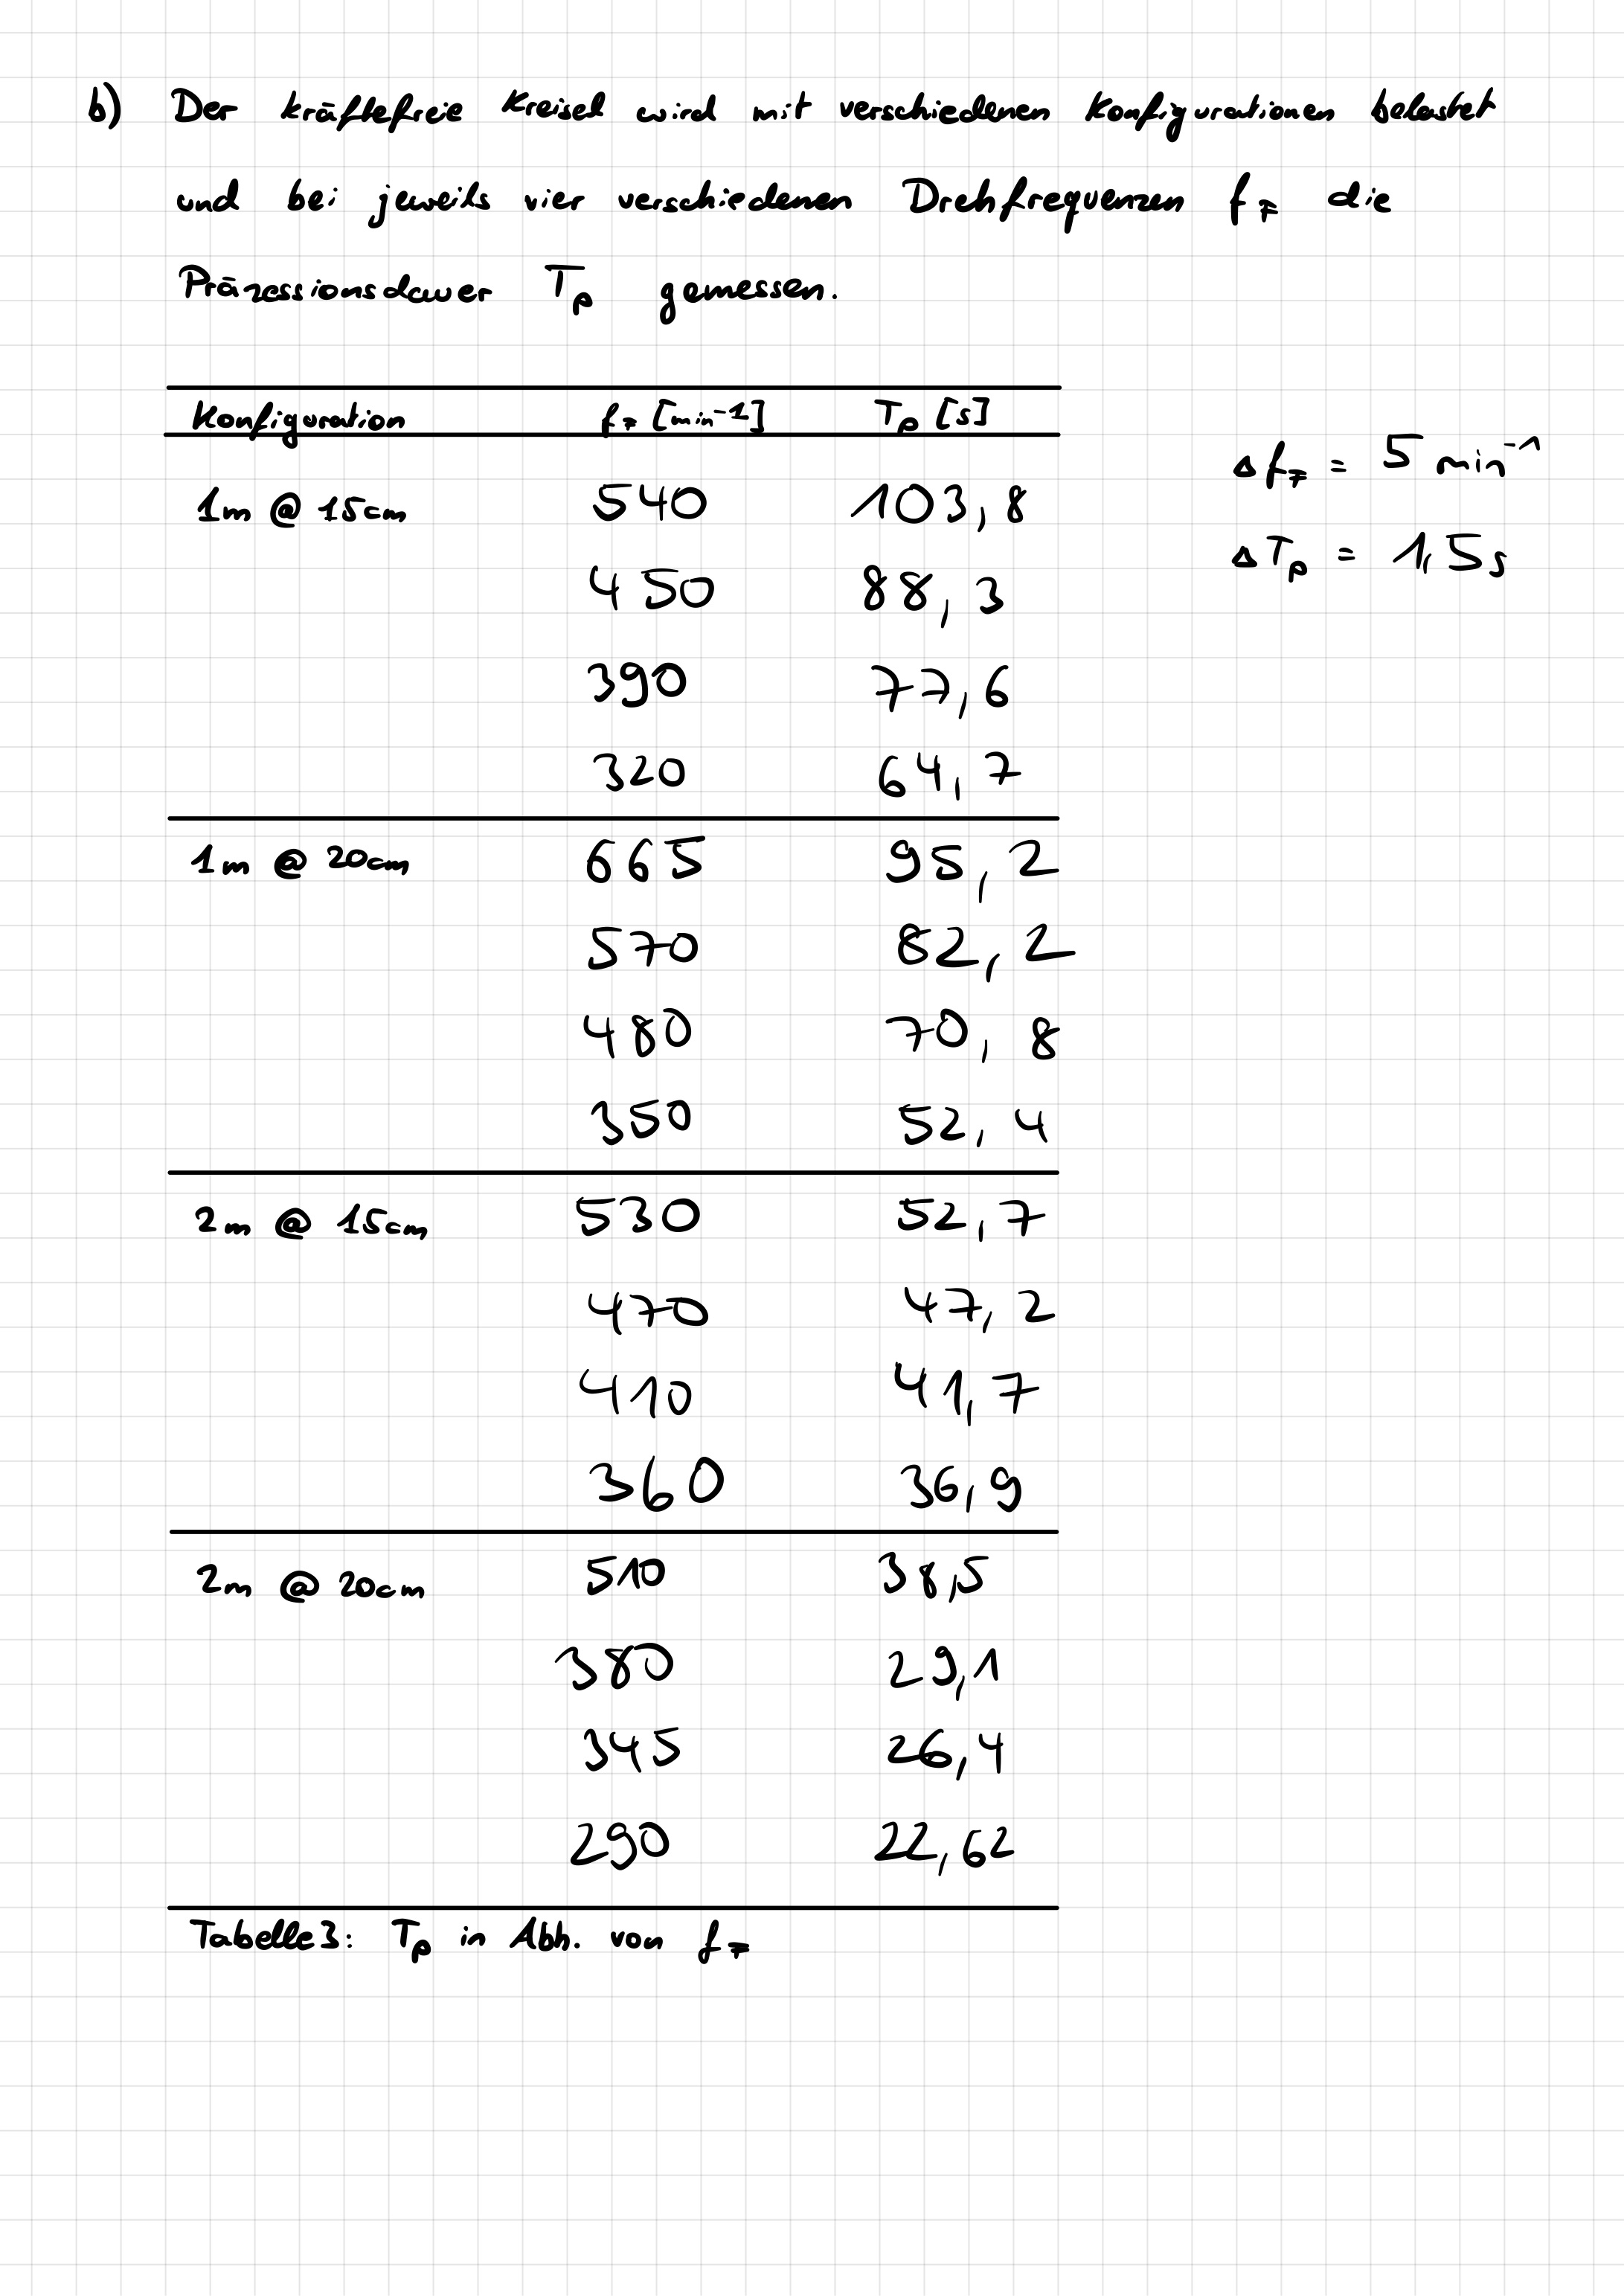
\includegraphics[width=\textwidth]{graphics/mess4.jpg}
\newpage
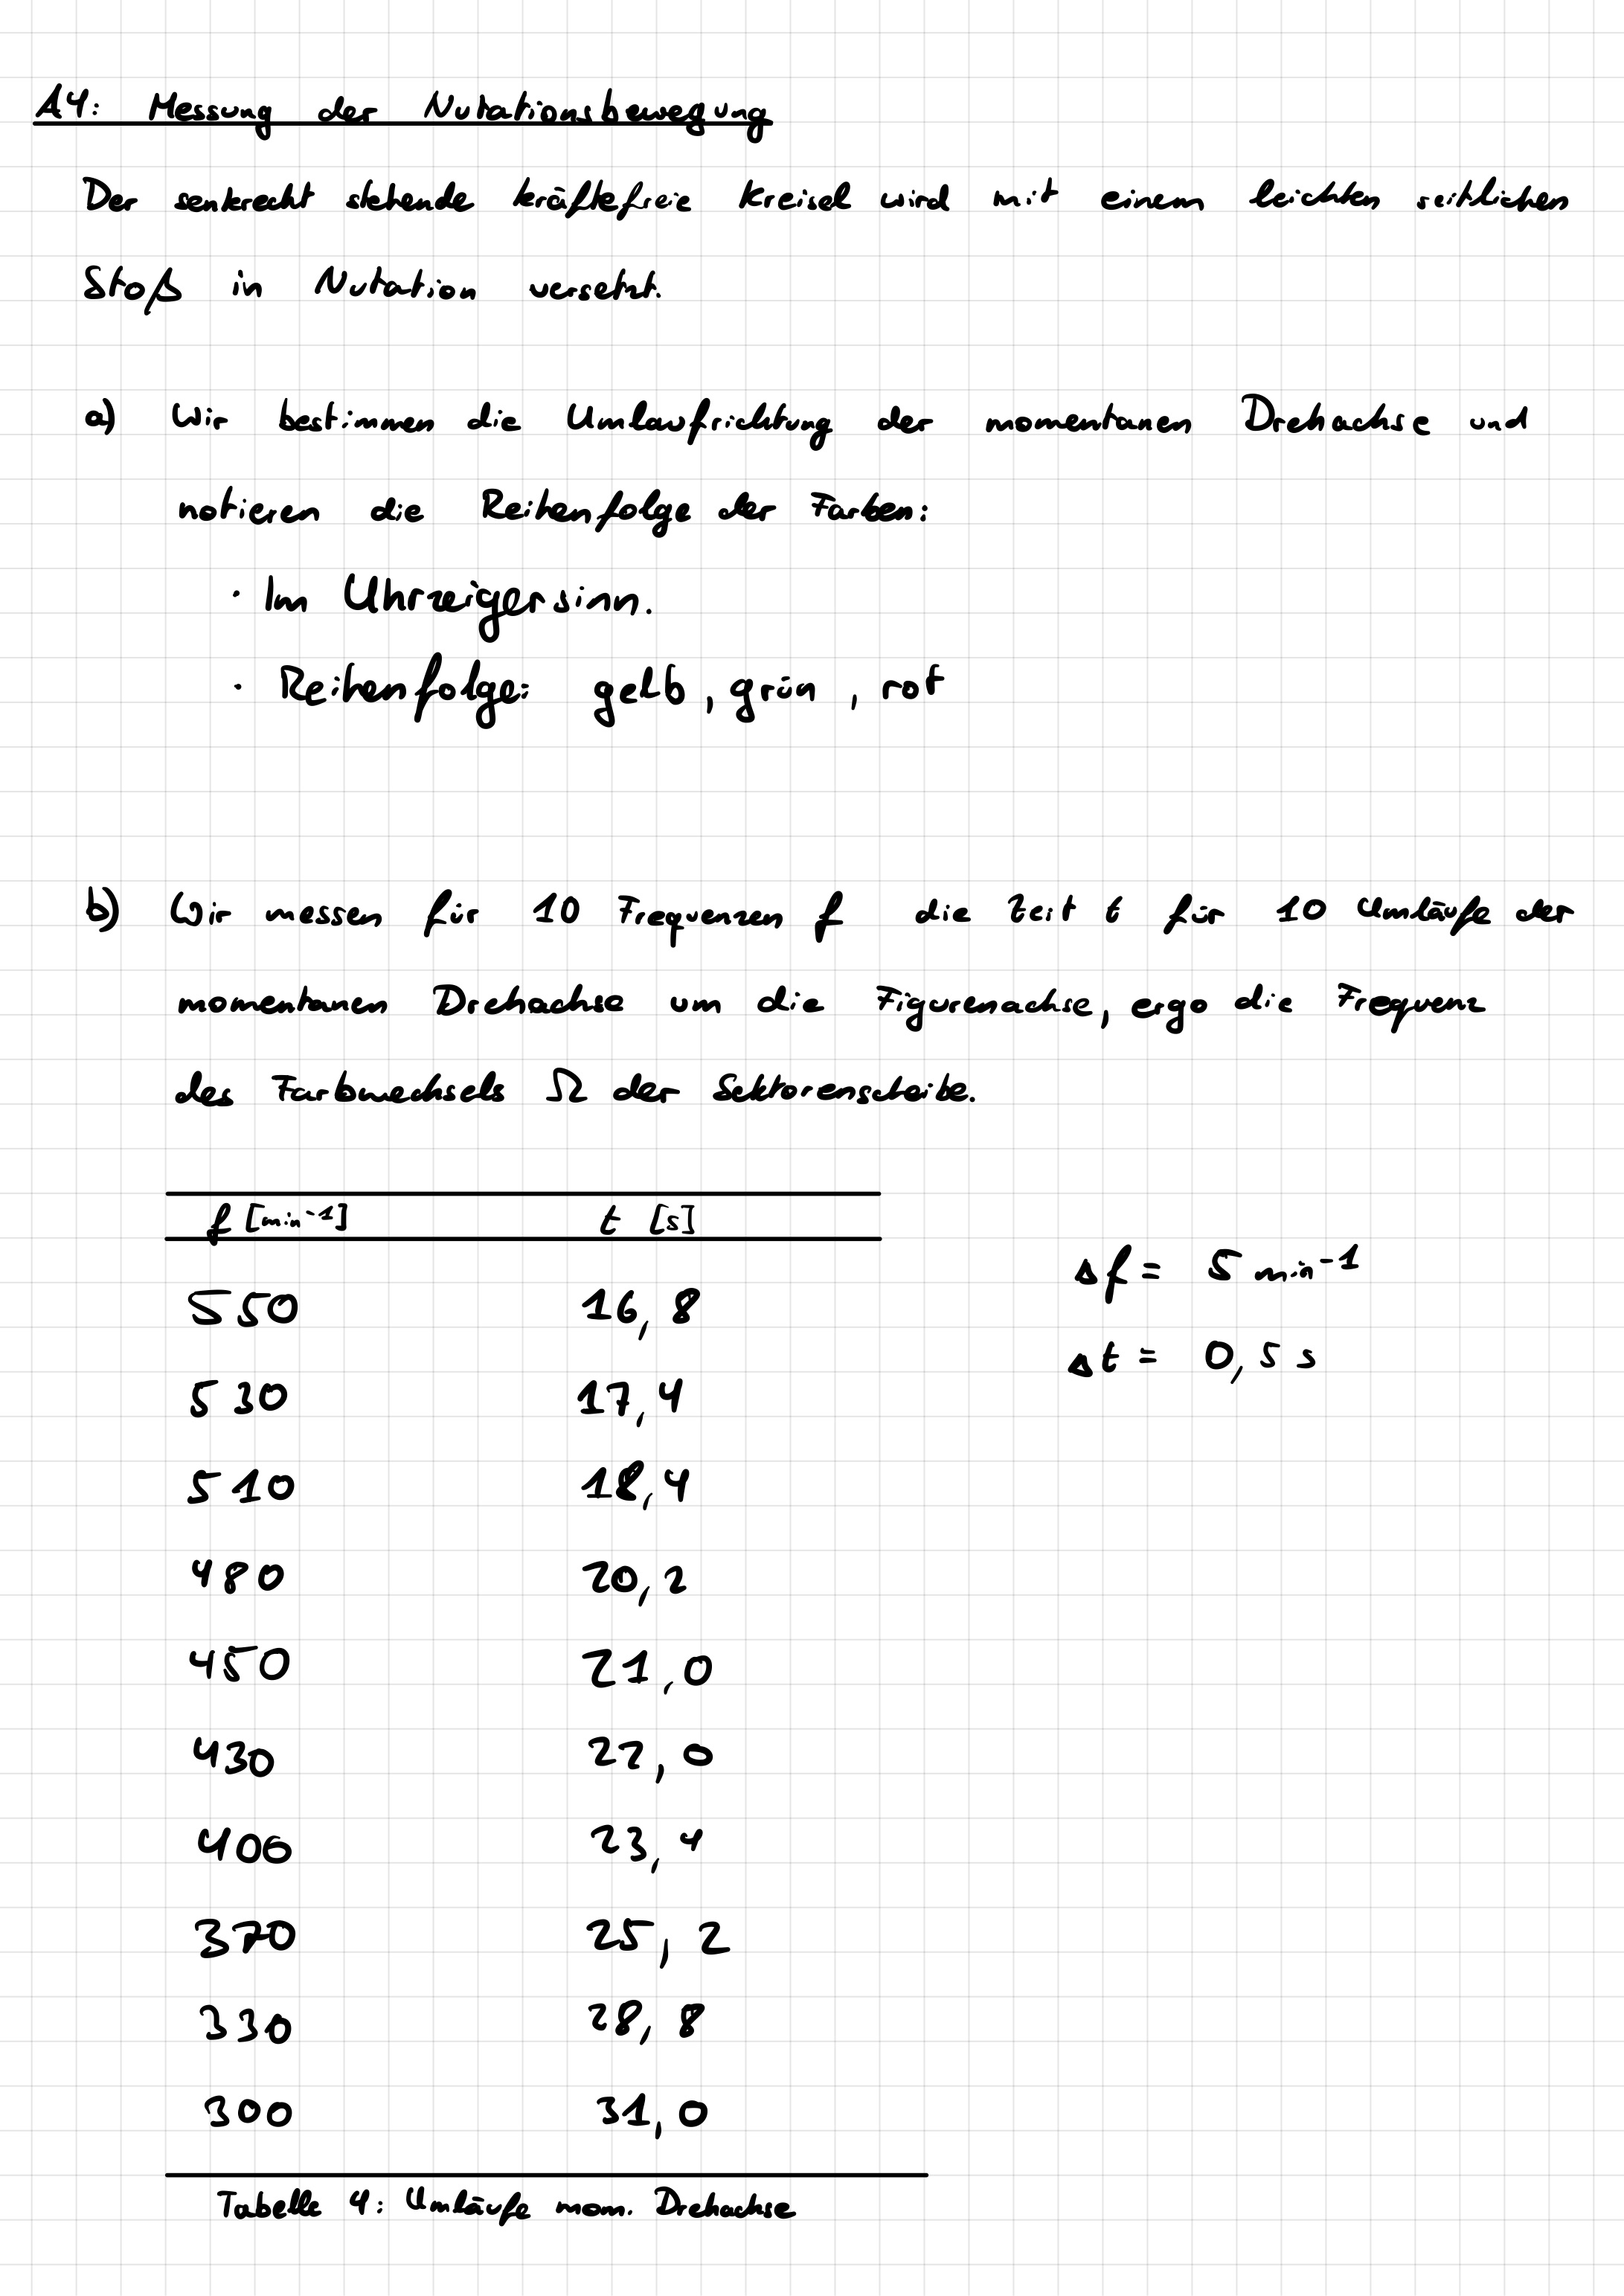
\includegraphics[width=\textwidth]{graphics/mess5.jpg}
\newpage
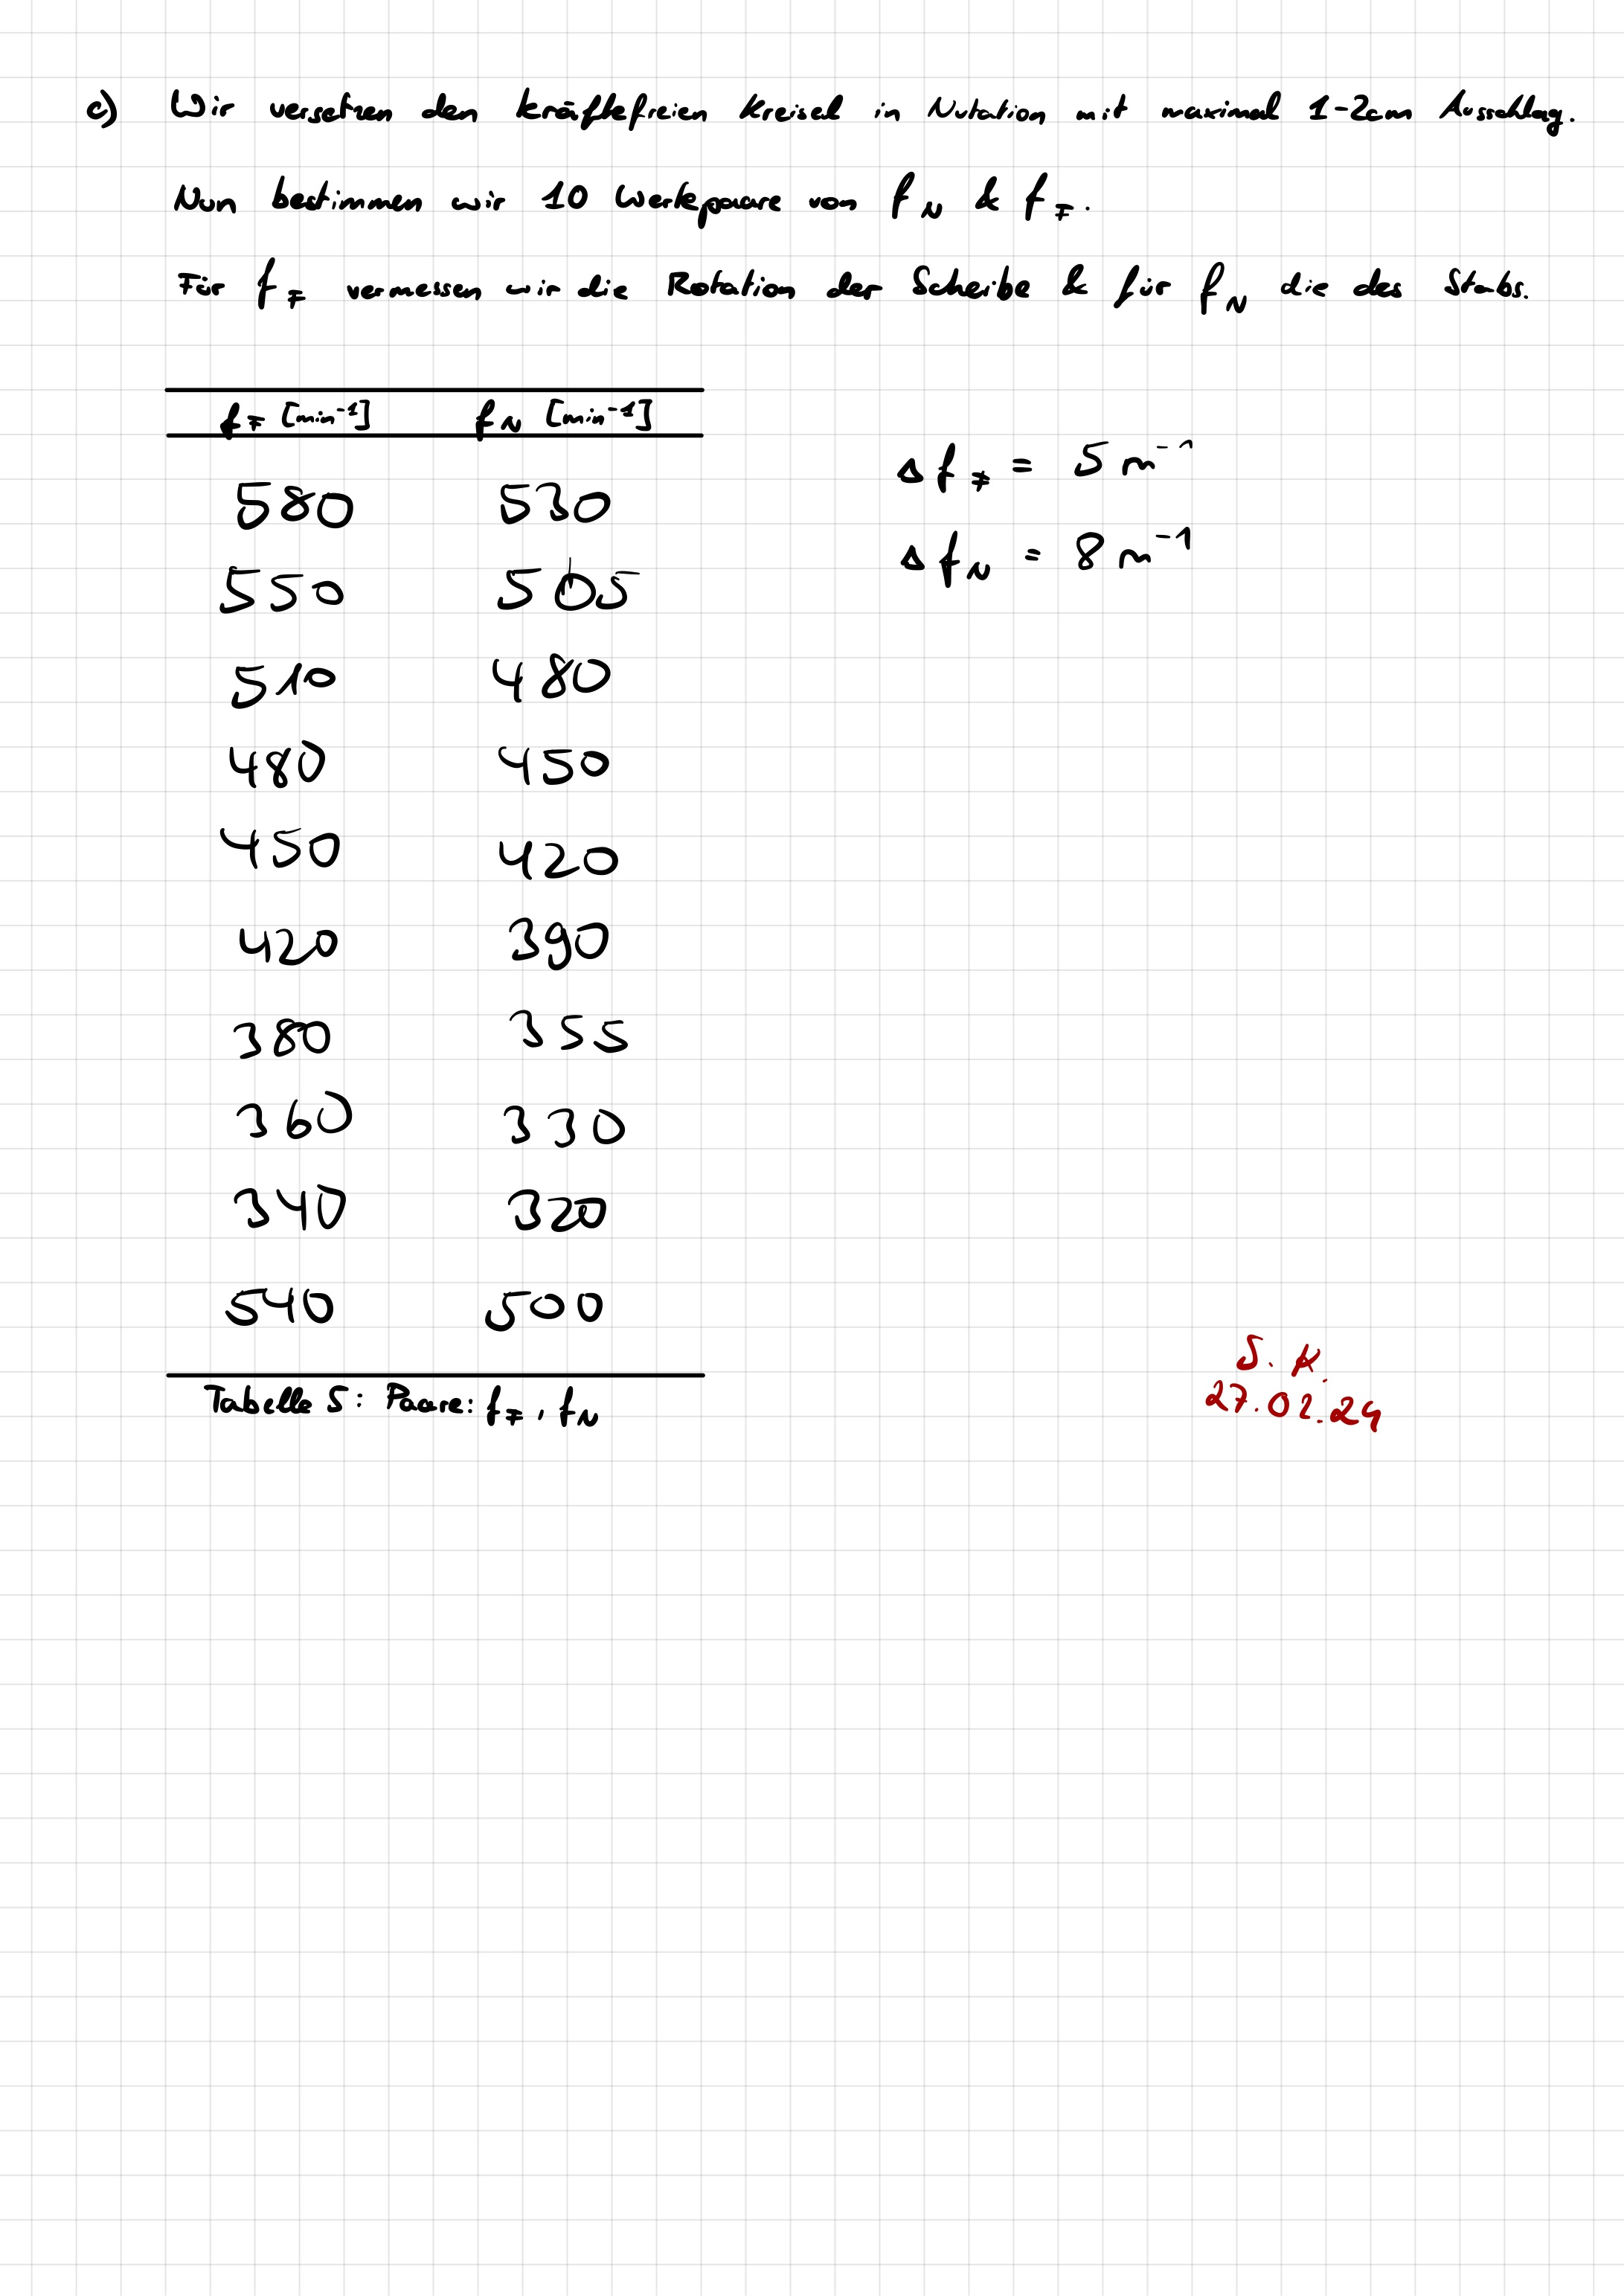
\includegraphics[width=\textwidth]{graphics/mess6.jpg}
\newpage

\addtocounter{table}{5}

\newpage
%-------------------------AUSWERTUNG-------------------------
\section{Auswertung}

In dieser Evaluation werden alle Fehler, sofern keine spezifische Angabe gemacht wird, mithilfe der Gauss'schen Fehlerfortpflanzung berechnet. Dies bedeutet, dass ein Wert $F$, der mit der Formel $f(a_1, ..., a_n)$ berechnet wird, den Fehler $\Delta F$ annimmt:

\begin{equation}
    \Delta F = \sqrt{\sum_n \left( \frac{\partial f}{\partial a_n} \cdot \Delta a_n \right)^2}.
\end{equation}

Des Weiteren erfolgen Signifikanztests von zwei Werten $a$ und $a'$ über die folgende Formel:

\begin{equation}
    \sigma = \frac{|a-a'|}{\sqrt{(\Delta a)^2 + (\Delta a')^2}}.
\end{equation}

Die Güte eines Fits wird mit der $\chi^2$-Summe bewertet:

\begin{equation}
    \chi^2 = \sum_i^N \left( \frac{\textit{Funktionswert}_i - \textit{Messwert}_i}{\textit{Fehler}_i} \right)^2
\end{equation}

Auch verwendet wird $\chi^2_{red} = \chi^2 / f$, wobei der Freiheitsgrad $f$ die Anzahl der Messwerte minus die Anzahl der Fitparameter ist. Der auf die Freiheitsgrade normierte Wert soll bei einem guten Fit ungefähr 1 sein.

Die Auswertung sowie Berechnung erfolgen über das dem Dokument angehängte Python-Programm.

\newpage

\subsection{Diskussion der Beobachtungen des Vorversuchs}

Im Versuchsteil a des Vorversuchs beobachteten wir den kräftefreien Kreisel bei zur Seite verschobener Figurenachse. Wir konnten feststellen, dass die Figurenachse des Kreisels stehenbleibt, wenn man diese möglichst Nutationsfrei loslässt, worauf sich schließen lässt, dass der Kreisel auch in diesem gekippten Zustand kräftefrei ist. Dies passt gut zu der theoretischen Erwartung. Der Kreisel ist trotz der Schieflage weiterhin im Schwerpunkt gelagert und somit wirkt kein zusätzliches äußeres Drehmoment, das eine Präzessionsbewegung auslösen könnte. 

Im zweiten Teil lösten wir durch leichtes Anschlagen der Figurenachse eine Nutationsbewegung aus. Auch hier konnten wir die erwarteten Beobachtungen feststellen. Deutlich zu erkennen war der Punkt der momentanen Drehachse, an dem die einzelnen Farben der Sektorenscheibe abwechselnd zu beobachten waren. Dies ist der Punkt, der in einem späteren Versuchsteil beobachtet wurde, um die Winkelgeschwindigkeit $\Omega$ der Nutation zu bestimmen, da die Farben hier mit dieser Geschwindigkeit wechseln. Auch bei der zweiten Scheibe mit den farbigen Ringen konnten die Erwartungen beobachtet werden. Je nach Anschlagsstärke erwischte man einen Nutationskegel auf einem der Farbringe oder eben nicht und je nachdem konnte man am Ort der momentane Drehachse eine konstante Farbe oder verwaschene Farben erkennen. Die konstante Farbe beim passenden Nutationskegel kommt hierbei davon, dass die Nutationsbewegung genau so kreist, dass immer eine Stelle im gleichem Abstand von der Figurenachse, ergo immer eine Stelle der gleichen Farbe, beim Punkt der momentanen Drehachse landet und es somit so aussieht, als sei die Farbe dort konstant.

Im Versuchsteil c beobachteten wir die Scheiben mit konzentrischen Kreisen. Zunächst die, bei der der Mittelpunkt der Kreise leicht vom Aufsetzpunkt versetzt ist. Hier konnte man ohne Nutation die verwaschenen Kreise um die Figurenachse erkennen, da die schnelle Drehung des Kreisels die verschobenen Kreise miteinander verschwimmen lässt, sodass es so wirkt, als wäre der Mittelpunkt der Kreise in der Drehachse. Bei der anderen Scheibe mit den genau zentrierten Kreisen wurde eine Nutationsbewegung ausgelöst. Man konnte beobachten, dass wieder der Mittelpunkt der verwaschenen Kreise in der raumfesten Drehimpulsachse zu liegen scheint. Grund hierfür ist die perfekt zentrierte konzentrische Kreisanordnung, die ähnlich wie bei Teil b mit der Ringscheibe dafür sorgt, dass bei passender Nutation immer ein gleicher Farbteil im Mittelpunkt liegt. Man kann sich diesen Fall auch als analoges Gegenstück zur ersten leicht versetzten Kreisscheibe vorstellen: Beim ersten rotierte die Scheibe mit versetzten Kreisen um eine feste Achse und beim zweiten rotiert eine feste Scheibe um eine durch die Notation versetzte Achse. Es ergibt sich also praktisch das gleiche Bild. Brachte man ein Zusatzgewicht am Stab an, so war die erwartete "girlandenförmige" Bewegung zu beobachten, ergo die Überlagerung von Nutation und Präzession.

Zuletzt beobachteten wir in Teil d die Abhängigkeit der Präzessionsrichtung von der Drehrichtung des Kreisels sowie der Position des Schwerpunkts zum Unterstützungspunkt. Für den Fall, dass der Schwerpunkt oberhalb der Kugelmitte lag konnten wir für eine Drehung des Kreisels im Uhrzeigersinn eine Präzession gegen den Uhrzeigersinn beobachten und bei Drehung gegen den Uhrzeigersinn eine Präzession im Uhrzeigersinn. Dementsprechend umgekehrt war es, wenn der Schwerpunkt unterhalb der Kugelmitte lag. Eine Drehung im Uhrzeigersinn bedeutete eine Präzession in dieselbe Richtung, genauso wie analog eine Drehung gegen den Uhrzeigersinn. Diese Umkehrung je nach Position des Schwerpunkts ergibt Sinn, da sich jeweils das Vorzeichen des zusätzlichen Drehmomentvektors umkehrt und so eine Kraft in die jeweils andere Richtung ausgeübt wird. Vergleichbar ist dies mit Abbildung \ref{fig:präzession}, wenn man sich vorstellt der Vektor $\Vec{l}$ zeige vom Kugelmittelpunkt nun nicht nach oben sondern nach unten.

Somit konnten im Vorversuch die Grundlagen des Kreisels analysiert werden und die theoretisch erwarteten Beobachtungen gemacht werden, eine perfekte Voraussetzung für die folgenden quantitativen Analysen. 

\newpage
\subsection{Bestimmung der Dämpfung und Halbwertszeit} \label{AuswertungDämpfung}

Wir möchten nun aus unseren Messungen von Versuchsteil 2 die Dämpfung durch die noch verbleibende Luftreibung quantitativ analysieren. Dazu berechnen wir zunächst aus den gemessenen Frequenzen $f$ aus Tabelle 1 des Messprotokolls die Drehfrequenzen $\omega = 2 \pi f$ und tragen diese in Abhängigkeit der Zeit in ein halblogarithmisches Diagramm auf. Daran fitten die Dämpfungsfunktion $\omega(t)$. Wir gehen von einem bekannten exponentiellen Verlauf aus und wählen somit

\begin{equation}
    \omega(t) = \omega_0 e^{- \delta t}.
    \label{eq:Dämpfungsfkt}
\end{equation}

Dies ist eine die Dämpfung beschreibende Funktion, die angibt, welche Drehfrequenz $\omega$ nach einer Zeit $t$ gemessen wird, wenn der Kreisel mit der Drehfrequenz $\omega_0$ startet und auf diesen die Dämpfungskonstante $\delta$ wirkt. Dabei berechnen sich durch den Fit die folgenden Werte:

\begin{equation}
    \begin{split}
        \omega_0 &= (63,42 \pm 0,28) \ \frac{\text{rad}}{\text{s}} \\
        \delta &= (0,749 \pm 0,012) \cdot 10^{-3} \ \text{s}^{-1}.
    \end{split}
\end{equation}

Man kann nun mit diesen Werten und Gleichung \ref{eq:Dämpfungsfkt} die Halbwertszeit bestimmen. Dazu setzt man $\omega(t_{\frac{1}{2}}) = \frac{\omega_0}{2}$ und stellt um nach $t_{\frac{1}{2}}$. Den Fehler bestimmt man anschließend nach dem Gauß'schen Fehlerfortpflanzungsgesetz. Man erhält:

\begin{equation}
    \begin{split}
        \frac{\omega_0}{2} &= \omega_0 e^{- \delta t_{\frac{1}{2}}} \\
        \iff t_{\frac{1}{2}} &= \frac{\ln{2}}{\delta} \\
        \Rightarrow \Delta t_{\frac{1}{2}} &= t_{\frac{1}{2}} \sqrt{\left( \frac{\Delta \delta}{\delta} \right)^2} \\ \\
        &\Rightarrow t_{\frac{1}{2}} = (925 \pm 15) \ \text{s}
    \end{split}
\end{equation}

Das generierte Diagramm mitsamt Fit und eingetragener Halbwertszeit ist in Abbildung \ref{plt:Daempfung} dargestellt. 

\phantom{.}

\begin{figure}[!h]
    \centering
    \resizebox{0.9\textwidth}{!}{
    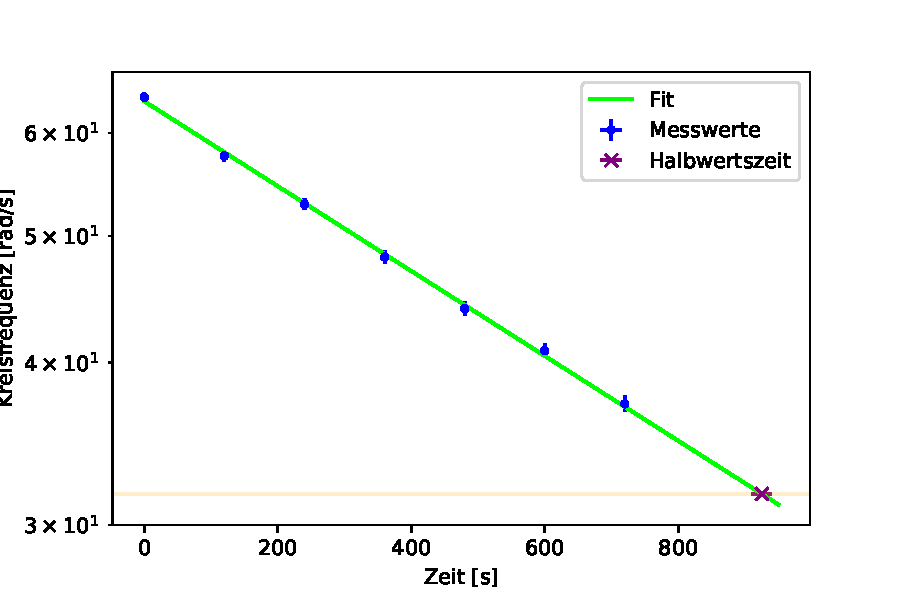
\includegraphics{graphics/plots/Daempfung.pdf}}
    \caption{Fit zur Bestimmung der Dämpfung inklusive Halbwertszeit}
    \label{plt:Daempfung}
\end{figure}

\phantom{.}

\clearpage
\newpage

\subsection{Auswertung der Präzessionsmessungen}

\subsubsection{Winkelabhängigkeit der Präzessionsdauer}

Zunächst betrachten wir die in Teil 3a durchgeführten Messungen der Präzessionsdauer bei verschiedenen Winkeln des Stabs. Wir vergleichen die Werte, indem wir Signifkanztests durchführen. Wir bekommen die folgenden Abweichungen:

\begin{equation}
    \begin{split}
        \sigma_{30,60} &= 0,4 \\
        \sigma_{30,90} &= 0,13 \\
        \sigma_{60,90} &= 0,6 \\
    \end{split}
\end{equation}

Wie wir sehen können, weichen alle drei Werte nur insignifikant voneinander ab. Dies lässt darauf schließen, dass die Präzessionsdauer und somit auch die Präzessionsbewegung im Gesamten unabhängig von dem eingestellten Winkel ist. Dies passt zu der in Kapitel \ref{Schw_Symm_Kreisel} hergeleiteten Unabhängigkeit der Präzessionsfrequenz von der räumlichen Orientierung des Kreisels. Kleinere Abweichungen der einzelnen Frequenzen lassen sich höchstwahrscheinlich darauf zurückführen, dass der Kreisel in der Praxis nicht perfekt nutationsfrei losgelassen werden kann und somit nie eine perfekte Präzessionsbewegung vorliegt.


\subsubsection{Berechnung des Trägheitsmoments $I_z$ aus der Präzession}

Wir beginnen, indem wir mit der in Kapitel \ref{AuswertungDämpfung} bestimmten Dämpfung für jede gemessene Präzessionsdauer die Drehfrequenz nach einer Präzession berechnen. Dazu verwenden wir die aus den in Tabelle 3 eingetragenen Frequenzen berechneten Drehfrequenzen $\omega_{F,i}$ als Startwerte $\omega_0$ und die gemssene Präzessionsdauer als Zeit, um den Wert der Drehfrequenz nach einer Präzession $\omega_{F,f}$ zu bestimmen. Für die Dämpfungskonstante $\delta$ verwenden wir den zuvor bestimmten Wert. Aus den zwei Werten der Drehfrequenz bestimmen wir dann die durchschnittliche Drehfrequenz $\overline{\omega}_m$. Die Fehler der Endwerte und der durchschnittlichen Werte berechnen sich dabei wie folgt:

\begin{equation}
    \begin{split}
        \Delta \omega_{F,f} &= e^{-\delta T_P} \sqrt{\left( \Delta \omega_{F,i} \right)^2 + \left( \omega_{F,i} T_P \cdot \Delta \delta \right)^2 + \left( \omega_{F,i} \delta \cdot \Delta T_P \right)^2} \\
        \Delta \overline{\omega}_m &= \frac{1}{2} \sqrt{(\Delta \omega_{F,i})^2 + (\Delta \omega_{F,f})^2}
    \end{split}
\end{equation}

Die Ergebnisse sind in Tabelle \ref{tab:w_m} mitsamt Fehler zu sehen.


\begin{table}[!h]
    \centering
    %\resizebox{\textwidth}{!}{
    \begin{tabular}{cccc}
        \hline
        \textbf{Kofiguration} & $\bm{\omega_{F,i}}$ [rad/s] & $\bm{\omega_{F,f}}$ [rad/s] & $\bm{\overline{\omega}_m}$  \\ \hline
         1M@15cm  &   56,5 $\pm$ 0,5 &  52,3 $\pm$ 0,5 &   54,4 $\pm$ 0,4 \\
                  &   47,1 $\pm$ 0,5 &  44,1 $\pm$ 0,5 &   45,6 $\pm$ 0,4 \\
                  &   40,8 $\pm$ 0,5 &  38,5 $\pm$ 0,5 &   39,7 $\pm$ 0,4 \\
                  &   33,5 $\pm$ 0,5 &  31,9 $\pm$ 0,5 &   32,7 $\pm$ 0,4 \\ \hline
         1M@20cm  &   69,6 $\pm$ 0,5 &  64,8 $\pm$ 0,5 &   67,2 $\pm$ 0,4 \\
                  &   59,7 $\pm$ 0,5 &  56,1 $\pm$ 0,5 &   57,9 $\pm$ 0,4 \\
                  &   50,3 $\pm$ 0,5 &  47,7 $\pm$ 0,5 &   49,0 $\pm$ 0,4 \\
                  &   36,7 $\pm$ 0,5 &  35,2 $\pm$ 0,5 &   35,9 $\pm$ 0,4 \\ \hline
         2M@15cm  &   55,5 $\pm$ 0,5 &  53,4 $\pm$ 0,5 &   54,4 $\pm$ 0,4 \\
                  &   49,2 $\pm$ 0,5 &  47,5 $\pm$ 0,5 &   48,4 $\pm$ 0,4 \\
                  &   42,9 $\pm$ 0,5 &  41,6 $\pm$ 0,5 &   42,3 $\pm$ 0,4 \\
                  &   37,7 $\pm$ 0,5 &  36,7 $\pm$ 0,5 &   37,2 $\pm$ 0,4 \\ \hline
         2M@20cm  &   53,4 $\pm$ 0,5 &  51,9 $\pm$ 0,5 &   52,6 $\pm$ 0,4 \\
                  &   39,8 $\pm$ 0,5 &  38,9 $\pm$ 0,5 &   39,4 $\pm$ 0,4 \\
                  &   36,1 $\pm$ 0,5 &  35,4 $\pm$ 0,5 &   35,8 $\pm$ 0,4 \\
                  &   30,4 $\pm$ 0,5 &  29,9 $\pm$ 0,5 &   30,1 $\pm$ 0,4 \\ \hline
    \end{tabular}%}
    \caption{Durchschnittliche Drehfrequenzen}
    \label{tab:w_m}
\end{table}


Wir fahren nun fort, indem wir für jede Konfiguration die gemessene Präzessionsdauer $T_P$ als Funktion der durchschnittlichen Drehfrequenz $\overline{\omega}_m$ in ein Diagramm auftragen und jeweils eine lineare Gerade durch den Ursprung anfitten, da wir aus den Steigungen der Geraden das Trägheitsmoment bestimmen können. Der in Abbildung \ref{plt:TPvsOmega_F} dargestellte Plot bestimmt die in Tabelle \ref{tab:I_z} notierten Steigungen $s_i$. Zusätzlich berechnen wir für jede Steigung direkt das Trägheitsmoment $I_z$ nach Gleichung \ref{eq:omegaP_omegaF}, wobei $l$ den Abstand der Massen vom Kreiselschwerpunkt und $m$ die Masse der angebrachten Gewichte ist, welche dem PAP2.1 Skript entnommen werden. Dabei wird der Längenfehler $\Delta l$ bei zwei Gewichten als die Höhe eines und bei einem Gewicht als die halbe Höhe eines Gewichts abgeschätzt. Wir verwenden also die Formeln \ref{eq:FehlerIz} und tragen die Werte auch in Tabelle \ref{tab:I_z} ein.

\begin{equation}
    \begin{split}
        \omega_P &= \frac{2 \pi}{T_P} = \frac{mgl}{I_z \omega_F} \\
        \Rightarrow I_z &= \frac{mgl}{2 \pi} \frac{T_P}{\omega_F} = \frac{mgl}{2 \pi} s_i \\
        \Rightarrow \Delta I_z &= I_z \sqrt{\left( \frac{\Delta l}{l} \right)^2 + \left( \frac{\Delta s_i}{s_i} \right)^2}
    \end{split}
    \label{eq:FehlerIz}
\end{equation}

\begin{table}[!h]
    \centering
    %\resizebox{\textwidth}{!}{
    \begin{tabular}{ccc}
        \hline
        \textbf{Kofiguration} & $\bm{s_i}$ [s$^2$/rad] & $\bm{I_z}$ [kg m$^2$] \\ \hline
         1M@15cm  & 1,934 $\pm$ 0,015 & 0,00446 $\pm$ 0,00017 \\
         1M@20cm  & 1,428 $\pm$ 0,009 & 0,00439 $\pm$ 0,00012 \\
         2M@15cm  & 0,978 $\pm$ 0,005 & 0,0045 $\pm$ 0,0003 \\
         2M@20cm  & 0,737 $\pm$ 0,004 & 0,00453 $\pm$ 0,00025 \\ \hline
    \end{tabular}%}
    \caption{Trägheitsmoment $I_z$ für jede Konfiguration}
    \label{tab:I_z}
\end{table}

\newpage

\begin{figure}[!h]
    \centering
    \resizebox{0.9\textwidth}{!}{
    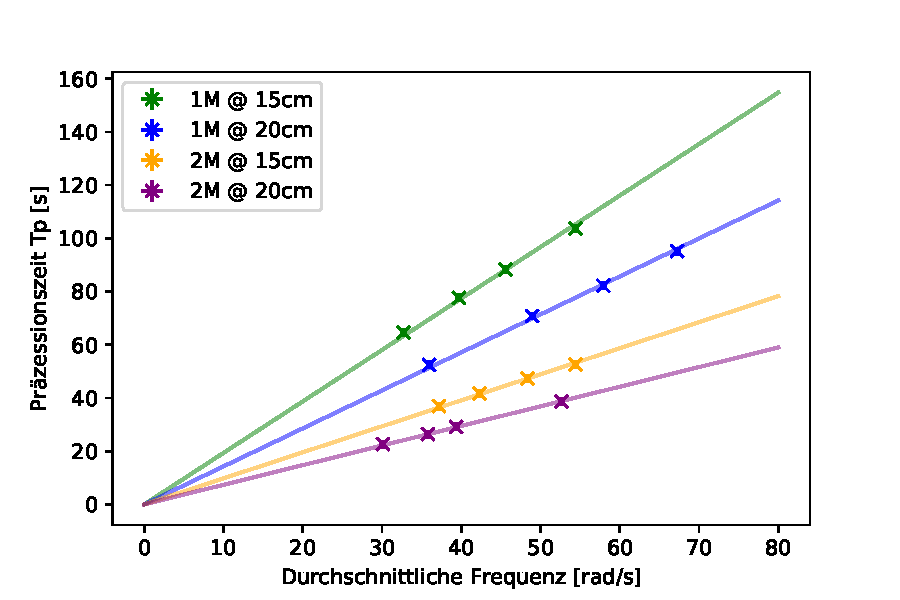
\includegraphics{graphics/plots/TPgegenOMEGA_F.pdf}}
    \caption{Lineare Fits aller Konfigurationen von $T_P$ gegen $\omega_F$}
    \label{plt:TPvsOmega_F}
\end{figure}

\phantom{.}


Aus den bestimmten Trägheitsmomenten bestimmen wir nun den Mittelwert $\overline{I}_z$ für unser Endergebnis. Der Fehler setzt sich zusammen aus dem Standardfehler des Mittelwerts $\sigma_{MW}$ sowie den Fehlern der Werte $\Delta I_{z,i}$:

\begin{equation}
    \Delta \overline{I}_z = \sqrt{(\sigma_{MW})^2 + \sqrt{\sum_i \left( \frac{\Delta I_{z,i}}{N} \right)^2}^2}.
\end{equation}

Somit erhalten wir als Endergebnis für das Trägheitsmoment des Kreisels:

\begin{equation}
    \overline{I}_z = (4,47 \pm 0,12) \cdot 10^{-3} \ \text{kg m}^2.
\end{equation}

Als Vergleichswert berechnen wir das theoretische Trägheitsmoment einer Kugel. Wir verwenden dazu die allgemeine Gleichung $I_K = \frac{2}{5} m r^2$ und setzten die im Skript gegebene Masse der Stahlkugel sowie deren Radius ein. Wir erhalten somit:

\begin{equation}
    I_{theo} = 4,2983 \cdot 10^{-3} \ \text{kg m}^2.
\end{equation}

Vergleichen wir die beiden Werte über einen Signifikanztest, so erhalten wir die Abweichung $\sigma_{I_z} = 1,5$. Dies liegt noch innerhalb der $3\sigma$-Umgebung und somit weicht der berechnete Wert nicht signifikant vom theoretischen Wert ab.


\newpage

\subsection{Auswertung der Nutationsbewegung}

\subsubsection{Vergleich der qualitativen Beobachtungen}

Wir konnten beobachten, dass sich die Figurenachse bei der Nutationsbewegung im Uhrzeigersinn dreht, was dieselbe Richtung ist, wie der Kreisel angedreht wurde. Dies passt auch zu dem in Abbildung \ref{fig:kräftefrei_symm_bew} dargestellten Fall. Zieht man Gleichung \ref{eq:WinkegeschwOmega} in Betracht, so kann man schlussfolgern, dass $I_x > I_z$ und $\omega_F > \Omega$ gelten muss.

\subsubsection{Bestimmung von $I_x$ über die Messung von $\Omega$}

Zunächst berechnen wir aus den gemessenen Zeiten für 10 Umläufe der momentanen Drehachse die Umlauffrequenz $\Omega = 2 \pi / (t/10)$. Die Ergebnisse werden in Tabelle \ref{tab:w_F-Omega} eingetragen. Der Fehler berechnet sich hierbei nach:

\begin{equation}
    \Delta \Omega = \frac{20 \pi}{t^2} \Delta t. 
\end{equation}

Auch tragen wir unsere gemessen Frequenzen $\omega_F$ der Figurenachse, natürlich wieder nachdem wir mit dem Faktor $2 \pi$ umgerechnet haben, in die Tabelle ein.

\phantom{.}

\begin{table}[!h]
    \centering
    %\resizebox{\textwidth}{!}{
    \begin{tabular}{ccc}
        \hline
        \textbf{Nr.} & $\bm{\omega_F}$ [rad/s] & $\bm{\Omega}$ [rad/s] \\ \hline
             1 &  57,6 $\pm$ 0,5 &     3,7 $\pm$ 0,5 \\
             2 &  55,5 $\pm$ 0,5 &     3,6 $\pm$ 0,5 \\
             3 &  53,4 $\pm$ 0,5 &     3,4 $\pm$ 0,5 \\
             4 &  50,3 $\pm$ 0,5 &     3,1 $\pm$ 0,5 \\
             5 &  47,1 $\pm$ 0,5 &     3,0 $\pm$ 0,5 \\
             6 &  45,0 $\pm$ 0,5 &     2,9 $\pm$ 0,5 \\
             7 &  41,9 $\pm$ 0,5 &     2,7 $\pm$ 0,5 \\
             8 &  38,7 $\pm$ 0,5 &     2,5 $\pm$ 0,5 \\
             9 &  34,6 $\pm$ 0,5 &     2,2 $\pm$ 0,5 \\
            10 &  31,4 $\pm$ 0,5 &     2,0 $\pm$ 0,5 \\ \hline
    \end{tabular}%}
    \caption{Frequenzen der Figurenachse $\omega_F$ \& Drehachse $\Omega$}
    \label{tab:w_F-Omega}
\end{table}

\phantom{.}

Wir nehmen nun diese Werte und tragen $\Omega$ gegen $\omega_F$ in ein Diagramm auf. Erneut fitten wir eine Gerade durch die Messwerte und bestimmen die Steigung. Der Fit, zu sehen in Abbildung \ref{plt:OMEGAvsOmega_F}, berechnet den Wert:

\begin{equation}
    s_{f,\Omega} = \frac{\Omega}{\omega_F} = (63,84 \pm 0,28) \cdot 10^{-3}.
\end{equation}

Wir betrachten nun Gleichung \ref{eq:WinkegeschwOmega} und stellen um nach $I_x$:

\begin{equation}
    \begin{split}
        I_x - I_z &= \frac{I_z}{\frac{\omega_F}{\Omega}-1} = \frac{I_z}{\frac{1}{s_{f,\Omega}}-1} \\
        \Rightarrow I_x &= \underbrace{\left( \frac{1}{\frac{1}{s_{f,\Omega}}-1} + 1 \right)}_{= \frac{1}{(1/s)-1}+ \frac{(1/s)-1}{(1/s)-1} = \frac{1/s}{(1/s)-1} = \frac{1}{1-s}} I_z \\
        \Rightarrow I_x &= \frac{1}{1-s_{f,\Omega}} I_z
    \end{split}
\end{equation}

Mit dieser Formel berechnet sich der Fehler wie folgt:

\begin{equation}
    \Delta I_x = \sqrt{\left( \frac{I_z}{(1-s_{f,\Omega})^2} \cdot \Delta s_{f,\Omega} \right)^2 + \left( \frac{1}{1-s_{f,\Omega}} \cdot \Delta I_z \right)^2}.
\end{equation}

Somit erhalten wir für das Trägheitsmoment $I_x$:

\begin{equation}
    I_{x,1} = (4,78 \pm 0,11) \cdot 10^{-3} \ \text{kg m}^2.
\end{equation}

Es ist zu erkennen, dass dieser Wert die theoretische Vorgabe $I_x > I_z$ erfüllt. Ebenso kann man in Tabelle \ref{tab:w_F-Omega} sehen, dass für alle Werte $\omega_F > \Omega$ gilt.

\begin{figure}[!hp]
    \centering
    \resizebox{0.9\textwidth}{!}{
    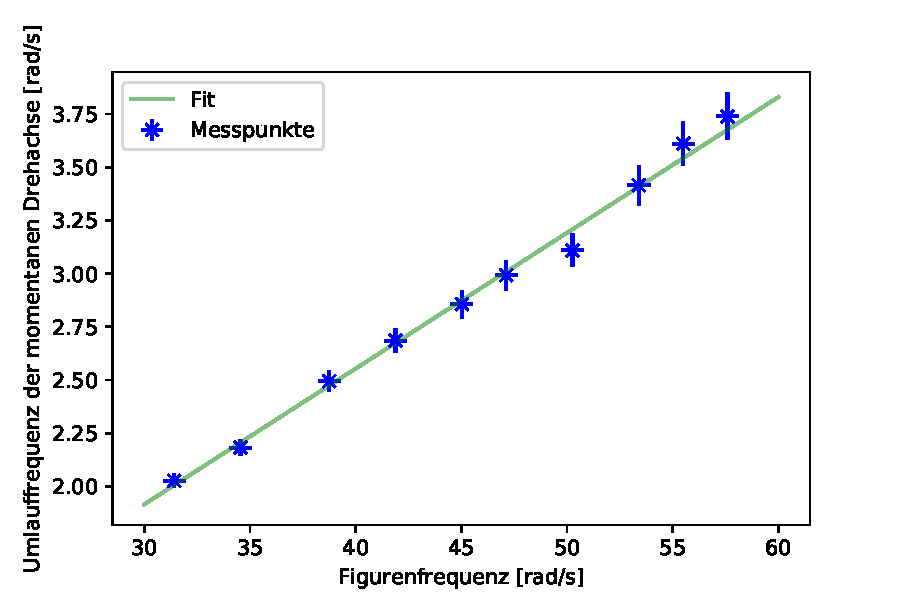
\includegraphics{graphics/plots/FitNutation1.pdf}}
    \caption{Plot der Messwerte $\Omega$ gegen $\omega_F$}
    \label{plt:OMEGAvsOmega_F}
\end{figure}

\clearpage
\newpage
\subsubsection{Bestimmung von $I_x$ über die Paare von $\omega_F$ und $\omega_N$}

Wir verwenden Gleichung \ref{eq:w_n-w_f} und stellen fest, dass wir, wenn wir $\omega_N$ als Funktion von $\omega_F$ in eine Diagramm eintragen, die Steigung der entstehenden Geraden gerade das Verhältnis $I_z/I_x$ ist. Wir tragen also die in Tabelle 5 gemessenen Wertepaare in ein Diagramm ein und fitten eine Gerade Funktion durch den Ursprung zu sehen in Abbildung \ref{plt:Omega_NvsOmega_F}. Wir erhalten somit die Steigung:

\begin{equation}
    s_{FN} = \frac{I_z}{I_x} = 0,927 \pm 0,003 .
\end{equation}

Erneut können wir so mit dem bereits bestimmten Wert für $\overline{I}_z$ den Wert von $I_x$ berechnen:

\begin{equation}
    \begin{split}
        I_x &= \frac{\overline{I}_z}{s_{FN}} \\
        \Delta I_x &= I_x \sqrt{\left( \frac{\Delta \overline{I}_z}{\overline{I}_z} \right)^2 + \left( \frac{\Delta s_{FN}}{s_{FN}} \right)^2} \\ \\
        &\Rightarrow I_{x,2} = (4,82 \pm 0,13) \cdot 10^{-3} \ \text{kg m}^2.
    \end{split}
\end{equation}

Diesen Wert vergleichen wir über einen Signifikanztest mit dem zuvor berechneten Wert $I_{x,1}$. Wir erhalten eine Abweichung von $\sigma_{I_x} = 0,25$. Somit liegt hier eine insignifikante Abweichung vor. Ebenso wirken die Werte $I_x$ sinnvoll im Kontext des betrachteten Kreisels, da bei einer Kugel mit dünnem Stab zu erwarten ist, dass sich die Trägheitsmomente für eine Drehung symmetrisch zum Stab ($I_z$) und senkrecht dazu ($I_x$) nicht allzu groß unterscheiden werden.

\begin{figure}[!hp]
    \centering
    \resizebox{0.9\textwidth}{!}{
    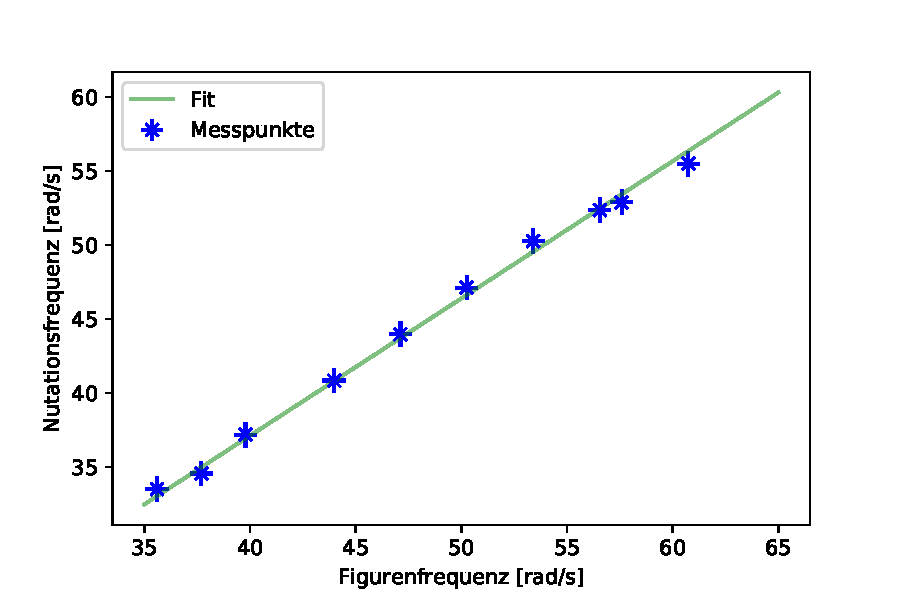
\includegraphics{graphics/plots/FitNutation2.pdf}}
    \caption{Plot der Messwerte $\omega_N$ gegen $\omega_F$}
    \label{plt:Omega_NvsOmega_F}
\end{figure}

\clearpage
\newpage
%---------------PRÄSENTATION DER ENDERGEBNISSE---------------
\section{Zusammenfassung der Endergebnisse}

Wir begannen, indem wir die Beobachtungen des Vorversuchs mit der Theorie abglichen. Wir untersuchten den kräftefreien und den schweren Kreisel sowie die Nutations- und Präzessionsbewegungen dieser. Hierbei wurden bei allen Teilen die erwarteten Beobachtungen gemacht. Das Verhalten des Kreisels, sei dies nun die Drehrichtung,  die Ausrichtung oder die beobachteten Scheiben, erfüllten immerzu die theoretischen Erwartungen und waren somit eine erste Bestätigung dieser.

Daraufhin bestimmten wir die Dämpfung des Kreisels, indem wir die Messung der Frequenz über 12 Minuten auswerteten und deren Abfall analysierten. Wir bestimmten daraus die Dämpfungskonstante $\delta$ sowie die Halbwertszeit $t_\frac{1}{2}$:

\begin{equation}
    \begin{split}
        \delta &= (0,749 \pm 0,012) \cdot 10^{-3} \ \text{s}^{-1} \\
        t_{\frac{1}{2}} &= (925 \pm 15) \ \text{s}
    \end{split}
\end{equation}

Anschließend werteten wir unsere Messungen der Präzessionsbewegung aus. Zunächst konnten wir erneut eine die Theorie bestätigende Beobachtung machen: Die Präzessionsbewegung ist unabhängig von der Orientierung des Kreisels! Dies wurde aus dem Vergleich der Messungen der Präzessionsdauer bei unterschiedlichen Neigungswinkeln des Kreisels hergeleitet, da sich alle nicht signifikant voneinander unterschieden. Anschließend nutzen wir unsere Messungen der Präzessionsdauer für verschiedenen Drehfrequenzen bei verschiednen Kofigurationen um das Trägheitsmoment $I_z$ des Kreisels zu bestimmen. Dazu trugen wir die Messwerte unter Berücksichtigung der zuvor bestimmten Dämpfung in eine Diagramm ein und nutzten die Steigungen der an die Werte angefitteten Geraden. Somit erhielten wir schlussendlich aus dem Mittelwert aller berchneten Trägheitsmomente den Wert:

\begin{equation}
    \overline{I}_z = (4,47 \pm 0,12) \cdot 10^{-3} \ \text{kg m}^2.
\end{equation}

Verglichen mit dem theoretischen Wert von $I_{theo} = 4,2983 \cdot 10^{-3}$kg m$^2$ ergab sich eine Abweichung von $\sigma_{I_z} = 1,5$. Dies ist nicht signifikant und zeigt somit, dass die Methode ein akkurates Ergebnis liefert, das die Theorie nicht verletzt. 

Im letzten Teil werteten wir unsere Beobachtungen und Messungen der Nutationsbewegungen aus, um im Endeffekt auf zwei verschiedene Weisen das Trägheitsmoment $I_x$ zu bestimmen. Doch zunächst konnten wir auch hier beobachten, dass sich der Kreisel so bewegte, wie es die Theorie vorhersagt. Spezifisch ging es um die Bewegungsrichtung der Nutationsbewegung, die in die selbe Richtung verlief wie der Kreisel insgesamt. Auch konnten wir die theoretischen Vorhersagen $I_x > I_z$ und $\omega_F > \Omega$ machen, welche sich beide in den darauffolgenden Abschnitten bestätigten.  

Zunächst bestimmten wir aus den Vermessungen der momentanen Drehachse den Wert:

\begin{equation}
    I_{x,1} = (4,78 \pm 0,11) \cdot 10^{-3} \ \text{kg m}^2.
\end{equation}

Anschließend verwendeten wir die gemessenen Wertepaare der Figuren- und Nutationsfrequenz und bestimmten damit:

\begin{equation}
    I_{x,2} = (4,82 \pm 0,13) \cdot 10^{-3} \ \text{kg m}^2.
\end{equation}

Ein Vergleich der beiden Werte für $I_x$ zeigt eine Abweichung von $\sigma_{I_x} = 0,25$. Es fühten also beide Wege zu verlässlichen Ergebnissen, die die Bedingung $I_x > I_z$ erfüllen und somit der Theorie nicht widersprechen.    

\newpage
%---------------ZUSAMMENFASSUNG UND DISKUSSION---------------
\section{Diskussion}

Aus der Zusammenfassung geht hervor, dass bei diesem Versuch weitreichend aussagekräftige, die Theorie bestätigende Ergebnisse erzielt werden konnten. Alle gemachten Beobachtungen waren immerzu erwartet und wurden bei genauerer Analyse von der Theorie unterstützt. Ebenso ergaben die berechneten Werte im Vergleich mit theoretischen Werten oder untereinander an jedem Punkt insignifikante Abweichungen beziehungsweise Sinn bei Gegenüberstellung. 

Für diese Ergebnisse wichtig war vor allem die Anfangs bestimmte Dämpfung, die bei den darauffolgenden Versuchsteilen die Ergebnisse deutlich verbessert haben wird. Betrachtet man beispielsweise in Teil 3b die Messungen der Präzessionsdauern, die teils bis zu knapp 2 Minuten dauerten und somit eine Frequenzdifferenz von bis zu etwa 4$\frac{\text{rad}}{\text{s}}$ beim Vergleich von Start- und Endwert ergaben, so wird klar, dass die Berücksichtigung wirklich nötig war. Ebenso war es gut, dass immer viele Messungen gemacht wurden. Seien das die verschiedenen Konfigurationen bei Teil 3b, die alle genutzt wurden um am Ende einen Wert für $I_z$ zu bestimmen, oder allgemein die jeweils 10 Messungen bei den Aufgabenteilen 4b \&c, so wurde das Endergebnis erheblich durch die Anzahl der Messungen verbessert. Im Gegenzug zeigen die Resultate der Auswertung dann, dass diese Anzahl an Messungen durchaus angebracht ist, da so konsistente und akkurate Ergebnisse erzielt werden konnten.  

Somit lassen sich bezüglich möglicher Verbesserungen des Versuchsaufbaus keine gröberen systematischen Fehler, sondern lediglich allgemeine Messfehler zur Motivation hinzuziehen. Ein Aspekt wäre natürlich, so wie immer bei manuellen Zeitmessungen, die Verbesserung der Genauigkeit durch technische Messgeräte wie Lichtschranken, die deutlich genauer die Präzessionsdauer oder Umlaufzeit in 4b bestimmen könnten. Ebenso wird einer der spürbarsten Fehlerquellen dieses Versuchs wohl die Frequenzmesung mit dem Stroboskop sein. Manuell die Lichtfrequenz akkurat an die Drehfrequenz anzupassen war häufig etwas mühevoll. Digitale Geräte, die automatisch bei Ausrichtung auf die Reflektorscheibe die Frequenz analysieren wären nicht nur genauer gewesen, sondern hätten zudem auch eine Echtzeit-Analyse und Berücksichtigung der Dämpfung ermöglicht, wenn diese durchgehend die Frequenz aufgezeichnet hätten. Somit wären nicht nur die Werte selbst besser gewesen, sondern auch die Korrektur der Dämpfung hätte profitiert. Ebenso wären mit solch einem Aufbau Messungen wie die in Teil 2, wo es gefordert war in bestimmten zeitlichen Abständen die Frequenzen zu bestimmen, deutlich einfacher, da die Messung der Frequenz mit dem Stroboskop durchaus eine Weile in Anspruch nimmt, bis die Frequenz angepasst wurde. Auch der letzte Teil, bei dem man möglichst schnell die Figuren- und Nutationsfrequenzen hintereinander bestimmen musste, hätte von solch einem System profitiert und das nicht nur wegen der generellen Mühsamkeit der Messung der Nutationsfrequenz anhand der Rotation des Stabs. Diese verflief nämlich auch sicherlich nicht allzu reibungslos, da es schwierig war unter Zeitdruck schnell den Stab zu fokussieren und die Anpassung der Frequenz hier auch nochmal zusätzlich etwas holpriger war. 

Dennoch lässt sich zusammenfassend sagen, dass alle Teile dieses Versuchs erwartete und miteinander im Einklang stehende Resultate erzielte. Somit war der Versuch eine lehrreiche Einführung in die komplexen Bewegungen von Kreiselsystemen, bei der mehrere zielsichere Methoden gezeigt wurden, diese zu Untersuchen und Analysieren.  

\newpage
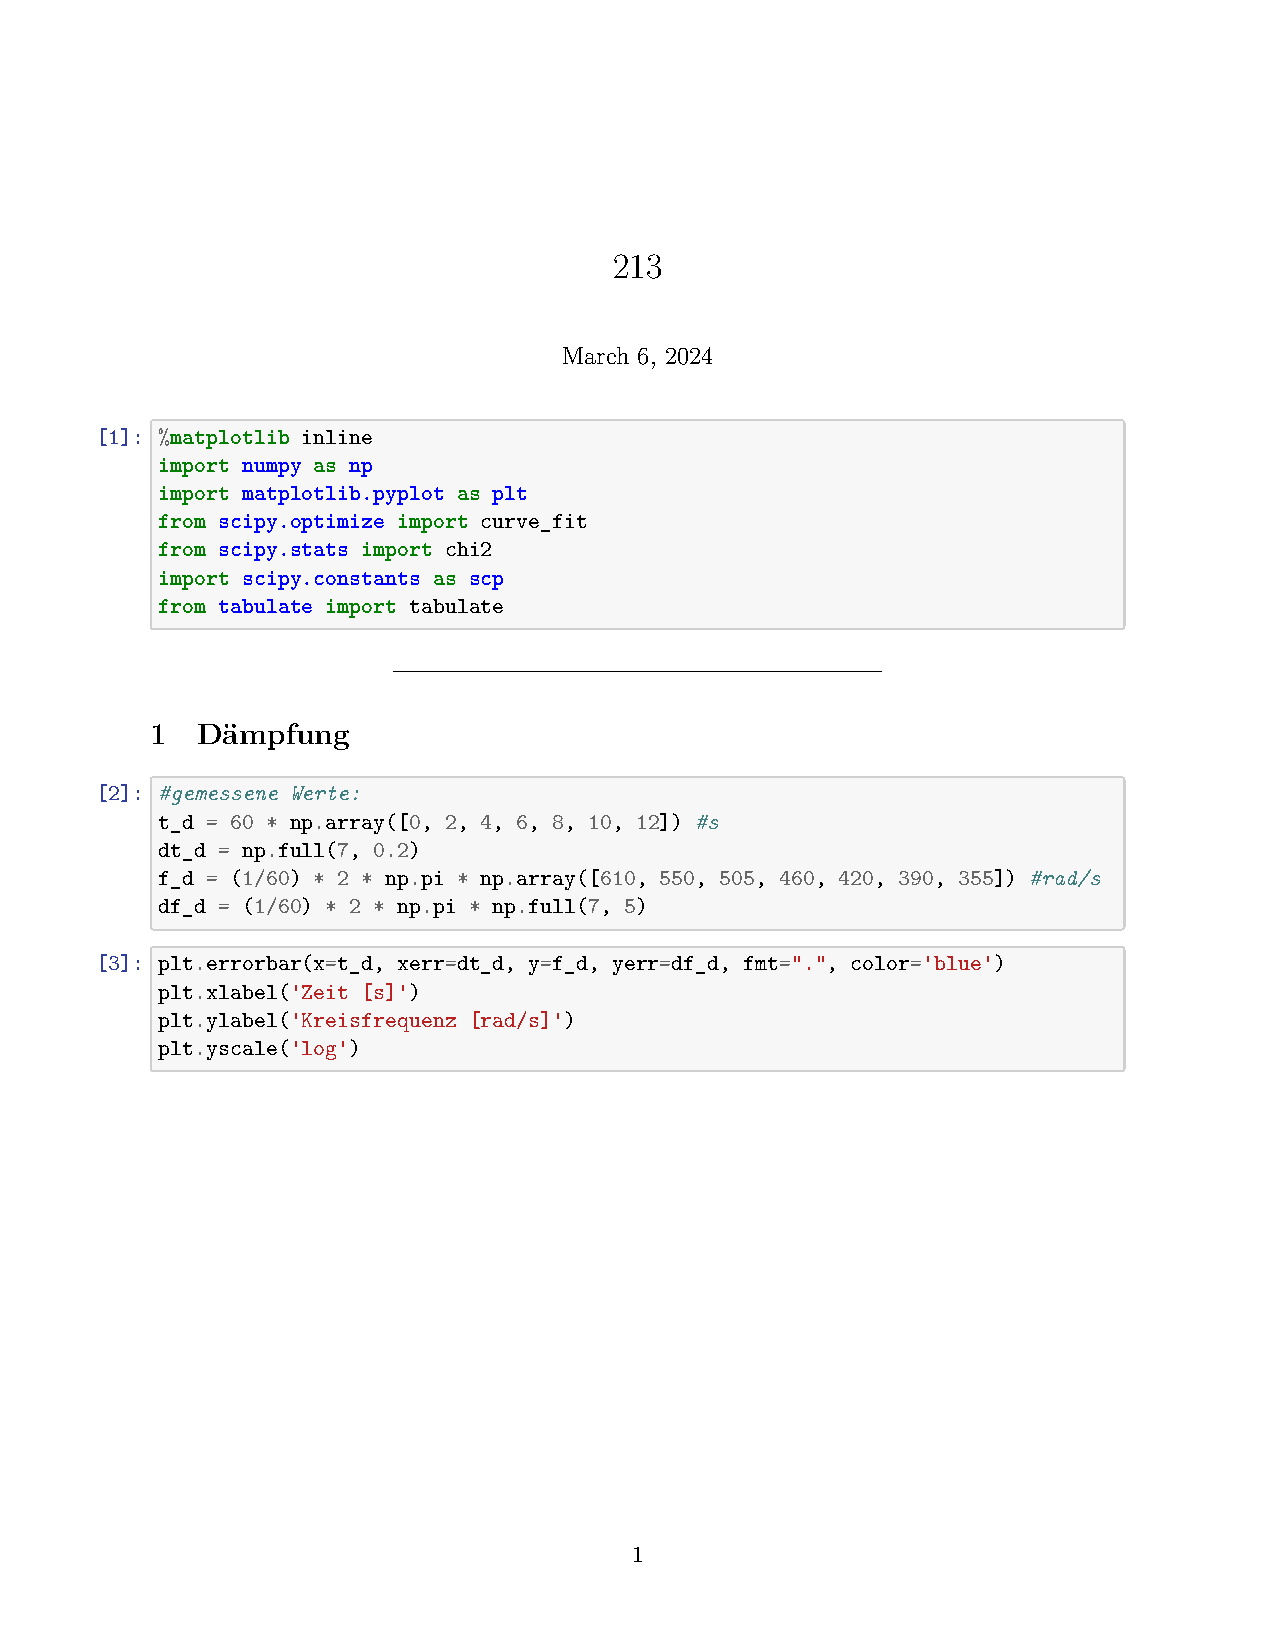
\includepdf[pages=-]{213.pdf}

\end{document}

